\documentclass[conference]{IEEEtran}
\usepackage{cite}
\usepackage{amsmath,amssymb,amsfonts}
\usepackage{algorithmic}
\usepackage{graphicx}
\usepackage{textcomp}
\usepackage{xcolor}
\usepackage{hyperref}
\usepackage{tikz}
\usepackage[utf8]{inputenc}
\usepackage{newunicodechar}
\usepackage{multirow}
\newunicodechar{₂}{$_2$}
\usetikzlibrary{shapes.geometric, arrows, positioning}

\usepackage{booktabs}


\usepackage{amsmath}
\usepackage{amsfonts}
\usepackage{algorithm}


\usepackage{caption}
\captionsetup[figure]{font=small, labelfont=bf} 

\hypersetup{
    colorlinks=true,     
    citecolor=blue,       
    linkcolor=blue,      
    urlcolor=blue         
}

\tikzstyle{startstop} = [rectangle, rounded corners, minimum width=3cm, minimum height=1cm,text centered, draw=black, fill=red!30]
\tikzstyle{io} = [trapezium, trapezium left angle=70, trapezium right angle=110, minimum width=3cm, minimum height=1cm, text centered, draw=black, fill=blue!30]
\tikzstyle{process} = [rectangle, minimum width=3cm, minimum height=1cm, text centered, text width=4cm, draw=black, fill=orange!30]
\tikzstyle{decision} = [diamond, minimum width=3cm, minimum height=1cm, text centered, text width=2cm, draw=black, fill=green!30]
\tikzstyle{arrow} = [thick,->,>=stealth]

\begin{document}

\title{Physics-Informed Double Deep Q-Networks for Scalable and Energy-Efficient Electric Vehicle Routing}

\author{\IEEEauthorblockN{1\textsuperscript{st} Given Name Surname}
\IEEEauthorblockA{\textit{Electrical Engineering} \\
\textit{Netaji Subhas University of Technology}\\
New Delhi, India \\
email address/ORCID}
}

\maketitle

\begin{abstract}
Lorem ipsum Lorem ipsum Lorem ipsum Lorem ipsum Lorem ipsum Lorem ipsum Lorem ipsum Lorem ipsum Lorem ipsum Lorem ipsum Lorem ipsum Lorem ipsum Lorem ipsum Lorem ipsum Lorem ipsum Lorem ipsum Lorem ipsum Lorem ipsum Lorem ipsum Lorem ipsum Lorem ipsum Lorem ipsum Lorem ipsum Lorem ipsum Lorem ipsum Lorem ipsum Lorem ipsum Lorem ipsum Lorem ipsum Lorem ipsum Lorem ipsum Lorem ipsum Lorem ipsum Lorem ipsum Lorem ipsum Lorem ipsum Lorem ipsum Lorem ipsum Lorem ipsum Lorem ipsum Lorem ipsum Lorem ipsum Lorem ipsum Lorem ipsum Lorem ipsum Lorem ipsum Lorem ipsum Lorem ipsum Lorem ipsum Lorem ipsum Lorem ipsum Lorem ipsum Lorem ipsum Lorem ipsum Lorem ipsum Lorem ipsum Lorem ipsum Lorem ipsum Lorem ipsum Lorem ipsum Lorem ipsum Lorem ipsum Lorem ipsum Lorem ipsum Lorem ipsum Lorem ipsum Lorem ipsum Lorem ipsum Lorem ipsum Lorem ipsum Lorem ipsum Lorem ipsum Lorem ipsum Lorem ipsum Lorem ipsum Lorem ipsum Lorem ipsum Lorem ipsum Lorem ipsum Lorem ipsum Lorem ipsum Lorem ipsum Lorem ipsum Lorem ipsum Lorem ipsum Lorem ipsum Lorem ipsum Lorem ipsum Lorem ipsum Lorem ipsum Lorem ipsum Lorem ipsum Lorem ipsum 
\end{abstract}

\begin{IEEEkeywords}
Electric Vehicle Routing, Double Deep Reinforcement Learning, Physics-Informed Neural Networks, Action Masking, SG-GAN
\end{IEEEkeywords}

\section{Introduction}


According to IPCC's Sixth Assessment Report 2022, 15\% of all global emissions (including direct and indirect sources) come from the global transportation sector, totalling roughly 8.9 GtCO₂ eq. Last-mile delivery fleets, which historically depend on diesel trucks, are a particular source of urban air pollution. In response, large logistics operators such as Amazon, DHL, and FedEx have begun replacing their conventional vans with electric vehicles to meet net-zero commitments \cite{b1}.

Large-scale transition modelling suggests that targeted cost-reduction policies could push EV market share to 70--85\% \cite{b2}, with corresponding reductions in operational energy use and tailpipe CO$_2$ across major markets. That shift, however, places a substantially higher load on electricity grids. Where renewable generation capacity grows more slowly than the EV fleet, net emissions may not fall as expected: the source of pollution moves from vehicle exhausts to the fossil-fuel power stations supplying the additional charging demand.

At the operational level, EVs introduce constraints that internal combustion vehicles do not face: restricted per-charge range, longer refuelling times, and sparse charging infrastructure. These constraints give rise to the Electric Vehicle Routing Problem (EVRP), whose core objective is to plan routes that minimise travel distance while guaranteeing the vehicle reaches a charging station before its battery is exhausted.

Tightening zero-emission regulations have pushed EVRP formulations well beyond simple distance minimisation; current models incorporate non-linear terms for payload, aerodynamic drag, and drivetrain losses \cite{b3}. Infrastructure is diversifying in parallel, with battery-swap depots, wireless inductive lanes, and mobile charging units entering the operational picture. Despite this progress, most published methods optimise a single objective, leaving multi-way trade-offs among battery degradation cost, station queue time, and carbon footprint largely unaddressed. Classical heuristic planners compound the problem further: because they cannot incorporate real-time traffic data, any unexpected congestion event forces a full route recomputation from scratch.

Reinforcement Learning is well suited to sequential routing decisions, but applying it to large road networks exposes two practical shortcomings: convergence slows considerably as the state space grows, and unconstrained agents routinely propose routes that violate hard energy limits, discovering the failure only after a stranding event occurs. This paper presents the PI-DDQN, which resolves both issues by folding longitudinal force equations directly into the action-selection step, so that infeasible moves are excluded before the agent ever considers them, and by decoupling the action-selection and value-estimation networks to suppress reward overestimation.

The paper is organized as follows: Section \ref{II} presents a literature review; Section \ref{III} describes the two-phase methodology of network generation and optimization; Section \ref{IV} formulates the results; Section \ref{V} details the computational experiment; Section \ref{VI} concludes the study.

\section{Literature Review}\label{II}

Building a deployable EV routing system involves at least three sub-problems that prior work has largely treated in isolation: constructing a road-network topology that is realistic enough for meaningful simulation, solving the combinatorial routing task under hard operational constraints, and computing per-step energy costs with sufficient accuracy to prevent vehicle stranding. The subsections below review where the literature stands on each front and where it falls short.

\subsection{Synthetic Map Generation and Topological Representation}
Any meaningful evaluation of a routing algorithm depends on the realism of the underlying road graph. Regular grid maps, the traditional proxy, fail to reproduce the node-degree variability, irregular edge lengths, and non-uniform connectivity found in real cities. Generative machine learning methods have consequently been proposed as a way to synthesise graphs whose statistical properties are closer to those of actual urban networks.

Das et al.\ combined a Spatial Graph-Generative Adversarial Network (SG-GAN) with tabular reinforcement learning to produce realistic mesh road topologies and demonstrated energy-use reductions in routed vehicles \cite{b4}. Separately, work pairing satellite imagery with explainable machine learning has shown that road-graph connectivity has a measurable effect on resource allocation and transport efficiency in urban settings \cite{b5}.

\subsection{EV Infrastructure Monitoring and Classical Heuristics}
Beyond graph generation, effective routing requires that CS allocation respects the operational constraints of the vehicle fleet. Early work in this domain was largely hardware-focused; for instance, centralized monitoring systems were deployed to measure power distribution across charging hubs \cite{b6}, with little consideration of dynamic vehicle demand.

Classical metaheuristic methods have since been applied to path-finding under hard operational boundaries. Wang et al.\ combined Genetic Algorithms with $A^*$ search to address the multi-objective EVRP under tight time windows \cite{b7}, while Xie et al.\ employed constraint-compliant initialization strategies to coordinate urban freight and energy delivery within battery and range limits \cite{b8}.

Despite their mathematical accuracy, classical heuristics cannot adapt to sudden traffic variations without entirely restarting their path-generation pipelines, making them impractical for real-time, in-car navigation systems.

\subsection{Data-Driven Deep Reinforcement Learning}
The inflexibility of classical optimization under dynamic conditions has motivated a shift toward Deep Reinforcement Learning (DRL), which frames routing as a sequential decision problem and learns adaptive policies through interaction with a simulated environment.

In the context of automated driving, Wu et al.\ demonstrated that DRL-based controllers can adapt speed and trajectory profiles in response to evolving traffic conditions, yielding measurable energy savings over fixed-policy baselines \cite{b9}. This work was extended to signalized intersection management, where deep Q-networks were trained to reduce stop-and-go energy losses in connected vehicle platoons \cite{b10}. 

At the macro-logistics scale, cooperative multi-agent reinforcement learning architectures have been developed to manage grid-aware EV charging distributions, deploying cross-site redirection rules to prevent localized grid failures while vehicles are moving \cite{b11}. Additionally, advanced Deep Q-Networks (DQN) have been built into adaptive cruise control systems to protect battery life during sudden stop-and-go traffic jams \cite{b12}.

\subsection{The Research Gap: The Need for PI-DDQN}
DRL resolves the state-space explosion that makes tabular methods impractical at scale, but two structural limitations persist in safety-critical routing scenarios:
\begin{itemize}
    \item \textbf{Value Overestimation:} A standard DQN uses the same network weights to both select and score a candidate route. The resulting upward bias in estimated Q-values causes the agent to repeatedly favour high-energy paths whose long-run cost has been overestimated, sometimes draining the battery before a charging station is reachable.
    \item \textbf{Physics-Blindness:} Networks trained purely on reward signals carry no representation of thermodynamic feasibility. A route can accumulate high reward in early episodes yet require more energy than the vehicle holds; the agent recognises the error only once a stranding penalty is incurred.
\end{itemize}

In logistics, a route that strands the vehicle mid-journey is a mission failure regardless of how well it performs on other metrics. Sun et al.\ incorporated physics-informed constraints into the training objective for stationary charging scheduling \cite{b13}, but that formulation was not designed for the sequential, on-road routing context addressed here.

No published method jointly handles real-time routing, dynamic congestion, and hard physical feasibility within a single learned policy. The PI-DDQN proposed here addresses all three through the following architectural decisions:

\begin{enumerate}
    \item \textbf{Decoupled Value Evaluation:} Action selection and value estimation are handled by separate networks following the Double DQN formulation \cite{van2016deep}, which removes the structural source of Q-value overestimation and keeps the agent from drifting toward energy-heavy corridors.
    \item \textbf{Physics-Informed Action Masking:} Before each decision step, the energy cost of every adjacent edge is computed from longitudinal force equations. Edges whose cost exceeds the vehicle's current SOC are masked out, so infeasible actions are excluded by construction rather than discouraged through penalisation after the fact.
    \item \textbf{Dynamic Congestion Integration:} Edge costs are updated after each traversal using the BPR flow-to-capacity ratio, scaling energy consumption with local vehicle density. This implicitly steers the agent away from saturated corridors without requiring an explicit traffic-prediction module.
\end{enumerate}

\section{Methodology} \label{III}
The proposed framework proceeds through three sequential phases. Phase~I uses an SG-GAN to synthesise a road network whose distributional properties match those of a real urban area, providing a controlled simulation environment that avoids the structural limitations of static grid graphs. Phase~II trains the PI-DDQN inside this environment, with thermodynamic constraints folded directly into the action-selection step. Phase~III specifies the physical energy and congestion model that produces the per-step cost signals the PI-DDQN is trained on.

\phantomsection
\subsection*{\textbf{Phase I: Environment Synthesis via SG-GAN}}
\addcontentsline{toc}{subsection}{Phase I: Environment Synthesis via SG-GAN}
The PI-DDQN is evaluated on topologies produced by an optimised SG-GAN \cite{das2025sggan}. Static historical graphs are insufficient for this purpose because they lack the structural variability required for robust policy evaluation \cite{kaufmann2020}. Standard GAN architectures \cite{goodfellow2014generative} handle continuous node-placement well but have documented difficulties with empirical edge-weight distributions and guaranteed graph connectivity \cite{you2018graphrnn, decao2018molgan}. Three modifications address these weaknesses in the version used here: \textit{Gradient Norm Clipping}, \textit{Direct Empirical Sampling}, and a \textit{Post-Hoc Heuristic KLD Search}. The generation pipeline is illustrated in Figure~\ref{fig:sg_gan_arch} and the corresponding hyperparameters are listed in Table~\ref{tab:gan_params}.

\begin{table}[htbp]
\caption{Optimized SG-GAN Hyperparameters}
\begin{center}
\renewcommand{\arraystretch}{1.4} % Adds uniform row padding
\begin{tabular}{|l|c|c|}
\hline
\textbf{Parameter Name} & \textbf{Symbol} & \textbf{Value} \\
\hline
Latent Noise Dimension & $z_{\text{dim}}$ & 10 \\
Training Epochs & $E_{\max}$ & 401 \\
Batch Size & $B$ & 32 \\
Adam Learning Rate & $\alpha$ & 0.0002 \\
Adam Betas & $(\beta_1, \beta_2)$ & $(0.5, 0.999)$ \\
Gradient Clipping Norm & $c$ & 5.0 \\
Connection Threshold & $\tau$ & 0.25 \\
\hline
\end{tabular}
\label{tab:gan_params}
\end{center}
\end{table}

\subsubsection{Adversarial Architecture and Optimization}
The core synthesis leverages a minimax adversarial game. The Generator ($G$) transforms latent noise vectors $z \sim \mathcal{N}(0, 1)$ into spatial graph node coordinates, while the Discriminator ($D$) attempts to differentiate these generated matrices from real geographical coordinate configurations extracted from the Dwarka Mor region in New Delhi. The networks optimize the Binary Cross-Entropy (BCE) objective:
\begin{equation}
\begin{aligned}
\min_{G} \max_{D} V(D, G) = \, & \mathbb{E}_{x \sim p_{\text{data}}(x)}[\log D(x)] \\
& + \mathbb{E}_{z \sim p_z(z)}[\log (1 - D(G(z)))]
\end{aligned}
\end{equation}


Spatial generation tasks are susceptible to mode collapse and gradient instability \cite{arjovsky2017wasserstein, salimans2016improved}. Both networks are optimized with Adam \cite{kingma2014adam}. To prevent gradient explosion, a known issue in GAN training on irregular graph data \cite{pascanu2013difficulty}, gradient-norm clipping is applied before each weight update. Specifically, the gradient vector $g = \nabla_\theta \mathcal{L}$ is rescaled whenever its $L_2$-norm exceeds the threshold $c = 5.0$: $\hat{g} = \min \left( 1, \frac{c}{||g||_2} \right) g$.

\begin{figure*}[ht]
\centering
\includegraphics[width=1\textwidth]{sggan_arch.png}
\caption{SG-GAN Architecture: Spatial Graph Generation for EV routing}
\label{fig:sg_gan_arch}
\end{figure*}

\subsubsection{Empirical Sampling and KLD-Minimized Edge Generation}
Instead of requiring the Generator to learn complex travel-speed distributions, our framework enforces realism through conditional empirical sampling. Based on authentic OpenStreetMap (OSM) telemetry \cite{haklay2008openstreetmap}, the network calculates the Haversine spatial distance $d_{u,v}$ \cite{sinnott1984virtues} between any two generated nodes $u$ and $v$. Edges are conditionally instantiated if the normalized distance falls below the threshold $\tau=0.25$.

To model realistic travel times $t_{u,v}$, the edge speed ratio $r$ is sampled directly from the empirical OSM distribution $R_{\text{real}}$, injected with Gaussian noise to preserve generative stochasticity \cite{daganzo1994cell}:
\begin{equation}
t_{u,v} = \frac{d_{u,v}}{\max(0.1, r + \mathcal{N}(0, \sigma^2))}
\end{equation}

The distributional fidelity of each synthesized graph is quantified using the Kullback-Leibler Divergence (KLD) \cite{kullback1951information} between the generated edge-speed distribution $P_{\text{fake}}$ and the OSM reference distribution $P_{\text{real}}$.

Baseline GAN topologies yield KLD values of $\sim0.54$, indicating substantial distributional mismatch. To address this, the framework runs a post-hoc heuristic search over $K=20$ candidate graphs generated from the same spatial node coordinates. Each candidate is conditionally connected and repaired for full graph connectivity via minimum-distance spanning. The topology with the lowest KLD, $G_{\text{best}} = \arg \min_{G_k} D_{\text{KL}}(P_{\text{real}} \| P_{G_k})$, is retained for use in simulation. This search reduces the KLD from $\sim0.54$ to \textcolor{red}{$\sim0.18$}, substantially improving the statistical alignment between the synthetic environment and real road network data. The integrated process is formally detailed in Algorithm \ref{algo:sg_gan}.

\begin{algorithm}[ht]
\caption{Optimized SG-GAN Synthesis with KLD Heuristic Search}
\label{algo:sg_gan}
\begin{algorithmic}[1]
\REQUIRE Real spatial coordinates $X_{\text{real}}$ and edge ratios $R_{\text{real}}$, Threshold $\tau=0.25$, Search iterations $K=20$
\ENSURE Topologically and statistically optimal synthetic network $G_{\text{best}}$
\STATE Initialize $G(\theta_G)$ and $D(\theta_D)$
\FOR{epoch = $1$ to $E_{\max}$}
    \STATE Sample real batch $x \sim X_{\text{real}}$ and noise $z \sim \mathcal{N}(0, 1)$
    \STATE Compute $\mathcal{L}_D$ and $\mathcal{L}_G$ via Minimax BCE
    \STATE Clip gradients $\hat{g} \leftarrow \min \left( 1, \frac{5.0}{||g||_2} \right) g$ for both networks
    \STATE Update $\theta_D, \theta_G$ using Adam Optimizer
\ENDFOR
\STATE Generate base coordinates $P \leftarrow G(z; \theta_G)$
\STATE $best\_KLD \leftarrow \infty$
\FOR{$k = 1$ to $K$}
    \STATE Initialize $G_{\text{temp}}$ over coordinates $P$
    \FOR{each spatial node pair $(u, v)$}
        \IF{Normalized Haversine distance $nd_{u,v} < \tau$}
            \STATE Sample $r \sim R_{\text{real}}$ and apply noise: $r_{\text{noisy}} \leftarrow \max(0.1, r + \mathcal{N}(0, 0.5))$
            \STATE Add edge $(u, v)$ with temporal cost $t_{u,v} = d_{u,v}/r_{\text{noisy}}$
        \ENDIF
    \ENDFOR
    \WHILE{$G_{\text{temp}}$ is disconnected}
        \STATE Bridge disjoint components via minimum-distance spanning
    \ENDWHILE
    \STATE Calculate $KLD \leftarrow D_{\text{KL}}(R_{\text{real}} || R_{G_{\text{temp}}})$
    \IF{$KLD < best\_KLD$}
        \STATE $best\_KLD \leftarrow KLD$, \quad $G_{\text{best}} \leftarrow G_{\text{temp}}$
    \ENDIF
\ENDFOR
\RETURN $G_{\text{best}}$
\end{algorithmic}
\end{algorithm}

\phantomsection
\subsection*{Phase II: Physics-Informed Double Deep Q-Network (PI-DDQN)}
\addcontentsline{toc}{subsection}{Phase II: Physics-Informed Double Deep Q-Network (PI-DDQN)}
\label{sec:pi_ddqn}
\setcounter{subsubsection}{0}

Two problems arise when standard RL is applied to large road networks. Tabular methods become intractable as network size grows because the state space expands exponentially \cite{sutton2018rl}. Both tabular and neural approaches also handle physical constraint violations retrospectively: an infeasible action must be taken, and a penalty incurred, before the policy updates to avoid it \cite{mnih2015dqn}. The PI-DDQN handles both issues within a single architecture. Neural function approximation keeps the method tractable as the graph scales; Double DQN target decoupling \cite{van2016deep, thrun1993issues} removes the overestimation bias that causes unconstrained agents to favour costly routes; and an energy-based mask blocks infeasible actions before selection rather than penalising them after.

\subsubsection{System Architecture and State Representation}
At each decision step $t$, the state observed by an EV navigating road graph $G(V,E)$ is encoded as:
\begin{equation}
\begin{aligned}
s_t = \left[\text{onehot}(v_t),\ \text{onehot}(v_{\text{dest}}),\ \frac{\text{SOC}_t}{\text{SOC}_{\max}}\right], \\
\dim(s_t) = 2|V| + 1.
\end{aligned}
\end{equation}
\textcolor{red}{For our scalable topologies (up to the 50-node maximum scale), the resulting 101-dimensional state vector is processed by a feedforward network with architecture $101 \rightarrow 128 \rightarrow 128 \rightarrow 50$ and ReLU activations \cite{goodfellow2016deep}.} The agent operates across three functional stages:
\begin{itemize}
    \item \textbf{Inference Flow:} The online Q-network ($\theta$) generates state-action values, which are immediately filtered by a physical safety mask. When an EV exhibits a critically low state of charge, a localized Bipartite Allocation protocol reassigns the vehicle to an optimal charging hub location \cite{kuhn1955hungarian}.
    \item \textbf{Training Loop:} Verified safe transitions are collected inside an experience replay buffer $\mathcal{D}$ \cite{lin1992self}. Random mini-batches ($b=64$) are extracted to update network parameters through an Adam optimizer \cite{kingma2014adam}, minimizing a composite loss function that explicitly penalizes trajectories violating physical boundaries.
    \item \textbf{Target Estimation:} The separate target Q-network ($\theta^-$) stabilizes expected value computations. Its parameters are periodically synchronized ($\theta^- \leftarrow \theta$) at designated intervals to suppress optimization divergence \cite{van2016deep}.
\end{itemize}

\subsubsection{Physics-Informed Action Masking and Optimization}
The central contribution of the PI-DDQN is the enforcement of energy feasibility constraints before, rather than after, each routing decision. At each step, the framework computes the energy demand $E_{\text{req}}(a)$ for every adjacent edge and constructs a binary action mask:
\begin{equation}
M(s_t, a) = 
\begin{cases}
0, & \text{if } \text{SOC}_t \ge E_{\text{req}}(a),\\
-\infty, & \text{otherwise.}
\end{cases}
\end{equation}
The effective Q-values are computed as $\tilde{Q}(s_t, a) = Q(s_t, a; \theta) + M(s_t, a)$, which drives the probability of selecting any energy-infeasible action to zero. Action selection then follows a masked $\epsilon$-greedy policy \cite{sutton2018rl}, ensuring exploration remains confined to the feasible action subset and battery depletion events are structurally prevented \cite{zhang2023ddqnper}.

Training minimizes a composite loss that combines the standard temporal difference error $\mathcal{L}_{\text{TD}}$ with an energy constraint penalty $\mathcal{L}_{\text{phys}}$:
\begin{equation}
\begin{aligned}
\mathcal{L} = \mathcal{L}_{\text{TD}} + \lambda \mathbb{E} \bigg[ \max \Big(0, \, & Q(s_t, a_t; \theta) \\
& - \big[ p_t + \gamma(1-d_t)\hat{Q}_{\text{next}} \big] \Big)^2 \bigg]
\end{aligned}
\end{equation}
where $p_t$ is the per-transition energy feasibility bound and $\lambda$ controls the relative weight of the physics penalty. This formulation draws on the PINN paradigm \cite{raissi2019pinn}, in which physical relationships are incorporated directly into the loss landscape rather than imposed solely through environment penalties.

\subsubsection{Shaped Reward Function}
To accelerate policy convergence and counter sparse terminal rewards, the environment updates the agent using a dense shaped reward function $r_t$:
\begin{equation}
\begin{aligned}
r_t = 10 - 5\left[\beta\frac{E_{ij}}{E_{\text{norm}}} + (1-\beta)\frac{t_{ij}}{T_{\text{norm}}}\right] - 2\delta_{ij} \\
{} + \mathbf{1}_{\text{dest}}\cdot 100 - \mathbf{1}_{\text{depleted}}\cdot 50 + \Delta\Phi(s_t)
\end{aligned}
\label{eq:reward}
\end{equation}
The trade-off parameter $\beta = 0.8$ prioritizes energy conservation over total travel time. The potential function $\Phi(s)$ incorporates A* shortest-path distance heuristics to smoothly guide the EV toward its target location, ensuring effective step-by-step guidance while preserving formal policy optimality guarantees \cite{ng1999policy}.

The internal mechanism of the reinforcement learning agent is depicted in Figure~\ref{fig:pi_ddqn_arch}, outlining the integration of physics-informed constraints within the loss calculation loop.

\begin{algorithm}[ht]
\caption{Multi-Agent PI-DDQN Routing with Physics Masking}
\label{algo:piddqn_detailed}
\begin{algorithmic}[1]
\REQUIRE Road graph $G(V,E)$, EV count $N$, replay capacity $B$, batch size $b$
\STATE Initialize online $Q(\theta)$, target $\hat{Q}(\theta^-)\leftarrow Q(\theta)$, replay buffer $\mathcal{D}$
\FOR{epoch $=1$ to $I_{\pi}$}
    \STATE Sample $N$ agents with random $(v_{\text{start}}, v_{\text{dest}}, \text{SOC}_0)$, initialize active set $\mathcal{A}$
    \FOR{step $=1$ to $T_{\max}$}
        \FOR{each agent $k\in\mathcal{A}$}
            \IF{$\text{SOC}_k \le T_h$}
                \STATE Reassign destination to the optimal minimum-cost charging station
            \ENDIF
            \STATE Compute energy demand $E_{\text{req}}(a)$ and apply mask $M(s_t, a)$
            \STATE Select action $a_t$ using masked $\epsilon$-greedy policy on $\tilde{Q}(s_t, a)$
            \STATE Execute transition: update congestion $\delta_{ij}$, energy $E_{ij}$, and $\text{SOC}_k$
            \STATE Store transition $(s_t,a_t,r_t,s_{t+1},d_t,p_t)$ in $\mathcal{D}$
        \ENDFOR
        \IF{$|\mathcal{D}| \ge b$}
            \STATE Sample mini-batch from $\mathcal{D}$ and compute DDQN targets $Y_t^{DDQN}$
            \STATE Minimize composite loss $\mathcal{L}_{\text{TD}}+\lambda\mathcal{L}_{\text{phys}}$ via Adam optimizer
        \ENDIF
    \ENDFOR
    \IF{epoch $\bmod \tau_{\text{sync}}=0$}
        \STATE Synchronize target network: $\theta^{-}\leftarrow\theta$
    \ENDIF
\ENDFOR
\end{algorithmic}
\end{algorithm}

\begin{figure*}[ht]
\centering
\includegraphics[width=1\textwidth]{piddqn_arch.png} 
\caption{Physics-Informed Double Deep Q-Network Architecture for Autonomous EV Routing}
\label{fig:pi_ddqn_arch}
\end{figure*}


\phantomsection
\subsection*{\textbf{Phase III: Calculation of Energy Consumption, Travel Time and Congestion}}
\addcontentsline{toc}{subsection}{Phase III: Calculation of Energy Consumption, Travel Time and Congestion}
\setcounter{subsubsection}{0}
The PI-DDQN evaluates environmental fitness through the explicit calculation of traction force, dynamic traffic congestion, and charging dwell times.

\subsubsection{Energy Consumption and Regenerative Braking}
The energy required to traverse an edge $(i, j)$ derives from fundamental longitudinal forces, including aerodynamic drag, rolling resistance, and road grade \cite{gillespie1992fundamentals, fiori2016power}:
\begin{equation}
F_{ij} = \frac{1}{2}\rho C_d A v_{ij}^{2} + C_r m g + m g \sin(\theta_{ij})
\end{equation}
The instantaneous mechanical power ($P_{ij} = F_{ij} \cdot v_{ij}$) is converted to electrical energy (kWh), accounting for a generic mechanical-to-electrical drivetrain efficiency ($\eta = 0.85$) \cite{ehsani2018modern}. In urban driving cycles, EVs recover energy during deceleration and descent. Our model explicitly incorporates regenerative braking, applying an efficiency factor of $0.80$ to establish the net free-flow energy cost \cite{settele2020peukert}:
\begin{equation}
E_{\text{net}, ij} = 0.80 \cdot \frac{F_{ij} \cdot d_{ij}}{\eta \cdot (3.6 \times 10^{6})}
\end{equation}

\subsubsection{Dynamic Congestion and Travel Time}
Traffic congestion non-linearly degrades energy efficiency. Following the principles of the Bureau of Public Roads (BPR) function \cite{bpr1964}, the dynamic congestion factor $\delta_{ij}$ reflects the real-time flow-to-capacity ratio:
\begin{equation}
\delta_{ij} = \min\left(1.0, \frac{q_{ij}}{C_{ij}}\right)
\end{equation}
The net energy consumption is mathematically inflated by this factor, scaling up to a 20\% penalty during absolute gridlock: $E_{\text{final}, ij} = E_{\text{net}, ij} (1 + 0.2 \delta_{ij})$. This efficiently mimics the stop-and-go energy drain and updates the vehicle's true $\text{SOC}_{t+1}$ \cite{das2025sggan}. Consequently, the PI-DDQN is actively incentivized to engage in network-wide load balancing.

The total traversal time $t_{ij}$ incorporates both congestion-induced delays and charging dwell times:
\begin{equation}
t_{ij} = t_{ij}^{\text{base}}\left(1 + 0.5 \delta_{ij}\right) + \frac{B_{\max} - B_{\text{current}}}{\eta_s}
\end{equation}
Queueing delays at charging hubs are implicitly governed by Little's Theorem ($W = L / \lambda_{\text{rate}}$), modeled by augmenting the local $\delta_{ij}$ of incoming edges proportional to accumulated EVs \cite{little1961}. 
Network parameters are updated via experience replay \cite{lin1992self}, sampling uniformly from a fixed-capacity buffer to break temporal correlation between training transitions. The key training hyperparameters are listed in Table~\ref{tab:training_hyperparameters}.

\begin{table}[htbp]
\centering
\caption{Training Hyperparameters}
\label{tab:training_hyperparameters}
\renewcommand{\arraystretch}{1.2}
\setlength{\tabcolsep}{6pt}
\small
\begin{tabular}{|l|c|p{4.3cm}|}
\hline
\textbf{Parameter} & \textbf{Value} & \textbf{Description} \\ \hline
Replay Memory ($B$) & 50,000 & Maximum capacity of stored transitions \\ \hline
Learning Rate & 0.001 & Adam Optimizer rate for weight updates \\ \hline
Batch Size & 64 & Samples pulled per training step \\ \hline
Physics Lambda ($\lambda$) & 0.5 & Weight of physics regularization in total loss \\ \hline
\end{tabular}
\end{table}

Taken together, these three sub-models produce a physically grounded cost signal at each transition step, requiring the PI-DDQN to simultaneously manage energy consumption, travel time, and charging station load without any of these objectives being specified as an explicit separate reward component.

\section{RESULTS AND DISCUSSION}
\label{IV}

All experiments used a mesh road network generated by the SG-GAN, comprising \textcolor{red}{35, 43, and 50 junction nodes (with 7, 9, and 10 charging stations respectively)}, and 50 EVs. Simulations ran in a Python-based Jupyter environment on a machine with an Apple M1 processor and 8~GB of RAM. The physical constants used in the energy model appear in Table~\ref{tab:physics_params}; the PI-DDQN hyperparameters are listed in Table~\ref{tab:piddqn_hyperparameters}.

\begin{table}[htbp]
\centering
\caption{Parameters Related to Energy Calculation}
\label{tab:physics_params}
\renewcommand{\arraystretch}{1.2} 
\setlength{\tabcolsep}{5pt}
\small
\begin{tabular}{|l|p{3.2cm}|c|}
\hline
\textbf{Parameter} & \textbf{Description} & \textbf{Value} \\ \hline
$\rho$ & Air density & 1.225 kg/m$^3$ \\ \hline
$C_d$ & Drag coefficient & 0.28 \\ \hline
$A$ & Frontal area of the vehicle & 2.3 m$^2$ \\ \hline
$C_r$ & Rolling resistance coefficient & 0.01 \\ \hline
$m$ & Mass of the EV & 1500 kg \\ \hline
$g$ & Acceleration due to gravity & 9.81 m/s$^2$ \\ \hline
$\eta$ & Mechanical to electrical efficiency & 0.85 \\ \hline
$\theta$ & Angle of the incline & 0$^\circ$--3$^\circ$ (random) \\ \hline
$I'$ & Congestion penalty multiplier & +20\% at $I'=1.0$ \\ \hline
\end{tabular}
\end{table}

\begin{table}[htbp]
\centering
\caption{PI-DDQN Model Configuration Hyperparameters}
\label{tab:piddqn_hyperparameters}
\renewcommand{\arraystretch}{1.15}
\setlength{\tabcolsep}{6pt}
\small
\begin{tabular}{|l|p{4.75cm}|c|}
\hline
\textbf{Parameter} & \textbf{Description} & \textbf{Value} \\ \hline
Network Type & Network used for experiments & Mesh \\ \hline
Initial Nodes & Initial number of nodes in the network & \textcolor{red}{35, 43, 50} \\ \hline
Maximum Episode & Cutoff training episode number & 800 \\ \hline
Learning Rate ($\alpha$) & Sets the Q-value update step size (Adam) & 0.0005 \\ \hline
Exploration & Initial exploration rate in $\epsilon$-greedy & 1.0 \\ \hline
Cutoff Exploration & Cutoff exploration rate in $\epsilon$-greedy & 0.05 \\ \hline
Gamma ($\gamma$) & Discount factor & 0.95 \\ \hline
Beta ($\beta$) & Weighting factor & 0.8 \\ \hline
Batch size & Replay buffer sample size & 64 \\ \hline
Physics ($\lambda$) & Penalty regularization weight & 0.25 \\ \hline
Replay Buffer & Experience replay capacity & 50,000 \\ \hline
$T_h$ & EV battery SOC threshold & 25\% \\ \hline
$B_{Max}$ & EV battery capacity & 10 kWh \\ \hline
\end{tabular}
\end{table}

\textcolor{red}{By scaling the node configurations, the SG-GAN produces three topologically distinct road networks (Fig.~\ref{fig:topologies}): a 35-node layout, a 43-node intermediate grid, and a 50-node dense urban structure. Each EV is assigned a 10 kWh battery with initial SOC sampled uniformly from $[30\%, 100\%]$, yielding a mean of 65\% and a standard deviation of 20.2\%.}

Vehicles are rerouted to the nearest charging station whenever their SOC falls below a 25\% safety threshold, equivalent to a 2.5 kWh reserve for the 10 kWh configuration. For larger battery capacities, this threshold scales proportionally: 16.7\% for 15 kWh, 12.5\% for 20 kWh, and 8.3\% for 30 kWh, preserving a consistent emergency buffer while avoiding unnecessarily frequent charging stops.

\subsection{Network Topology Validation}
\textcolor{red}{All three graph configurations were run under identical physical parameters so that any performance difference can be attributed to topological scale rather than to other experimental variables. The 50-node network increases the number of valid actions available at each node; the fact that PI-DDQN performance does not deteriorate on this configuration indicates that the policy generalises across varying connectivities without state-space degradation.}

\begin{figure}[htbp]
    \centering
    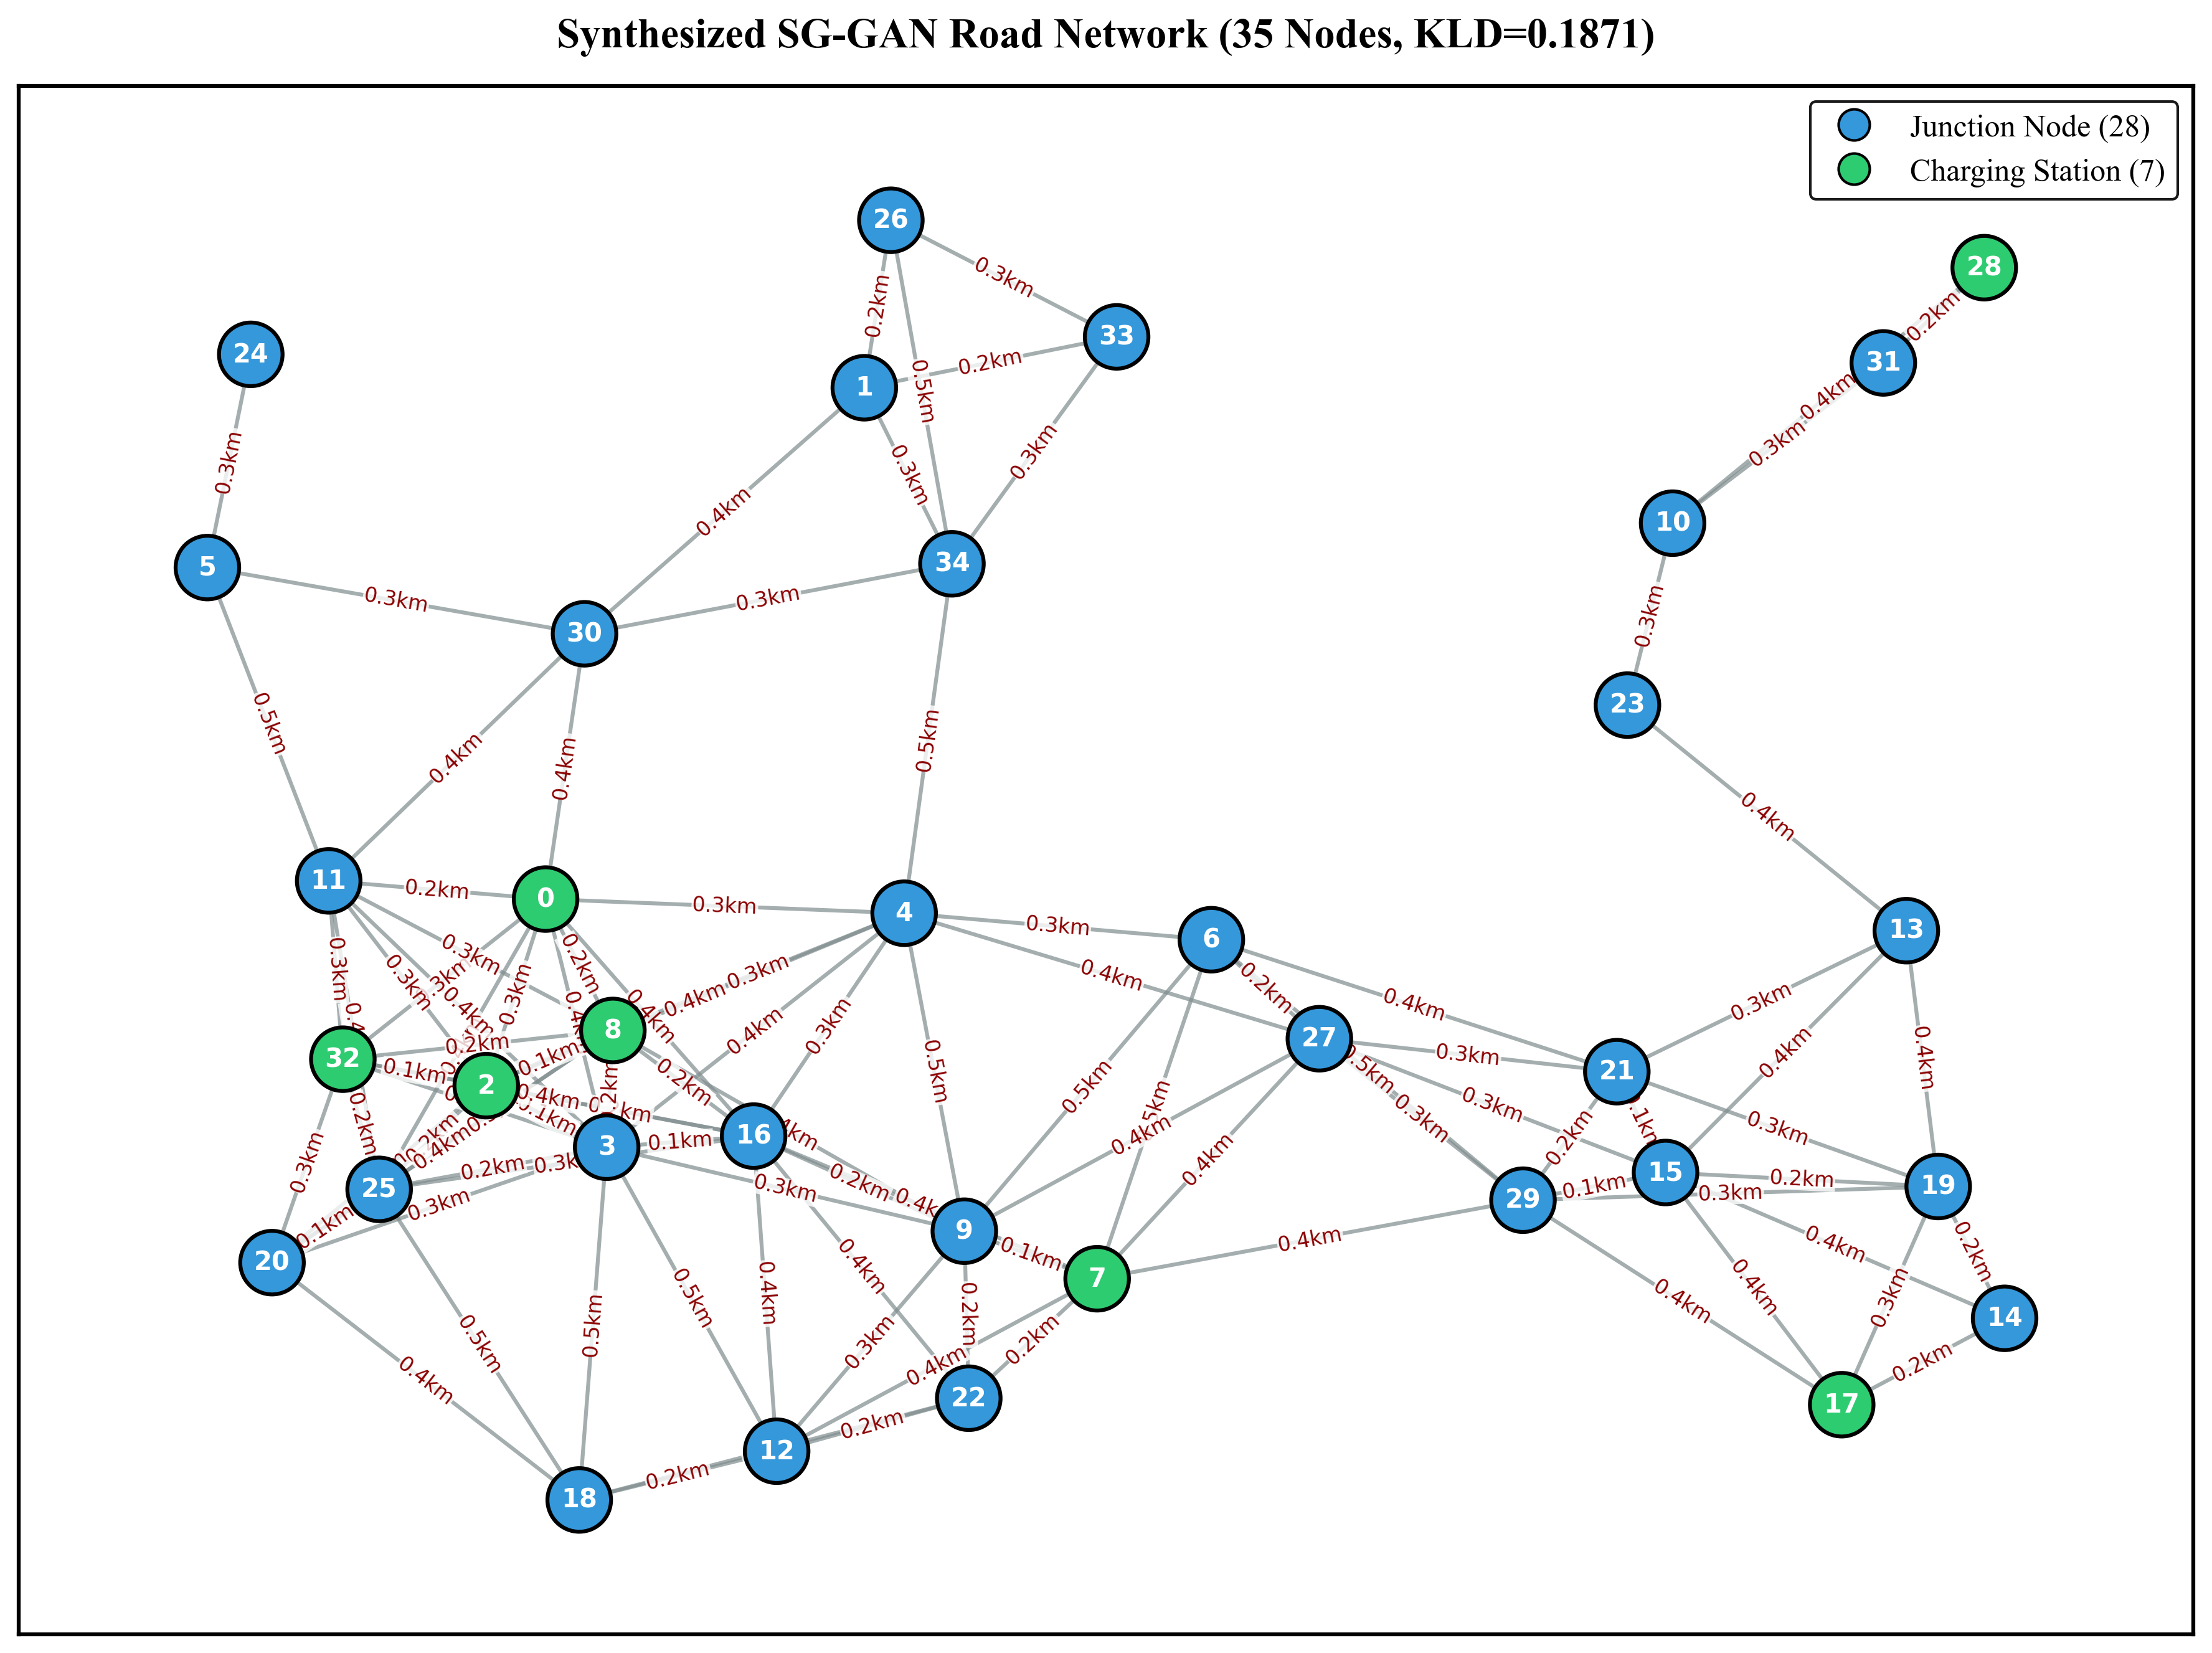
\includegraphics[width=0.48\columnwidth]{8a_Graph_35_nodes.png}
    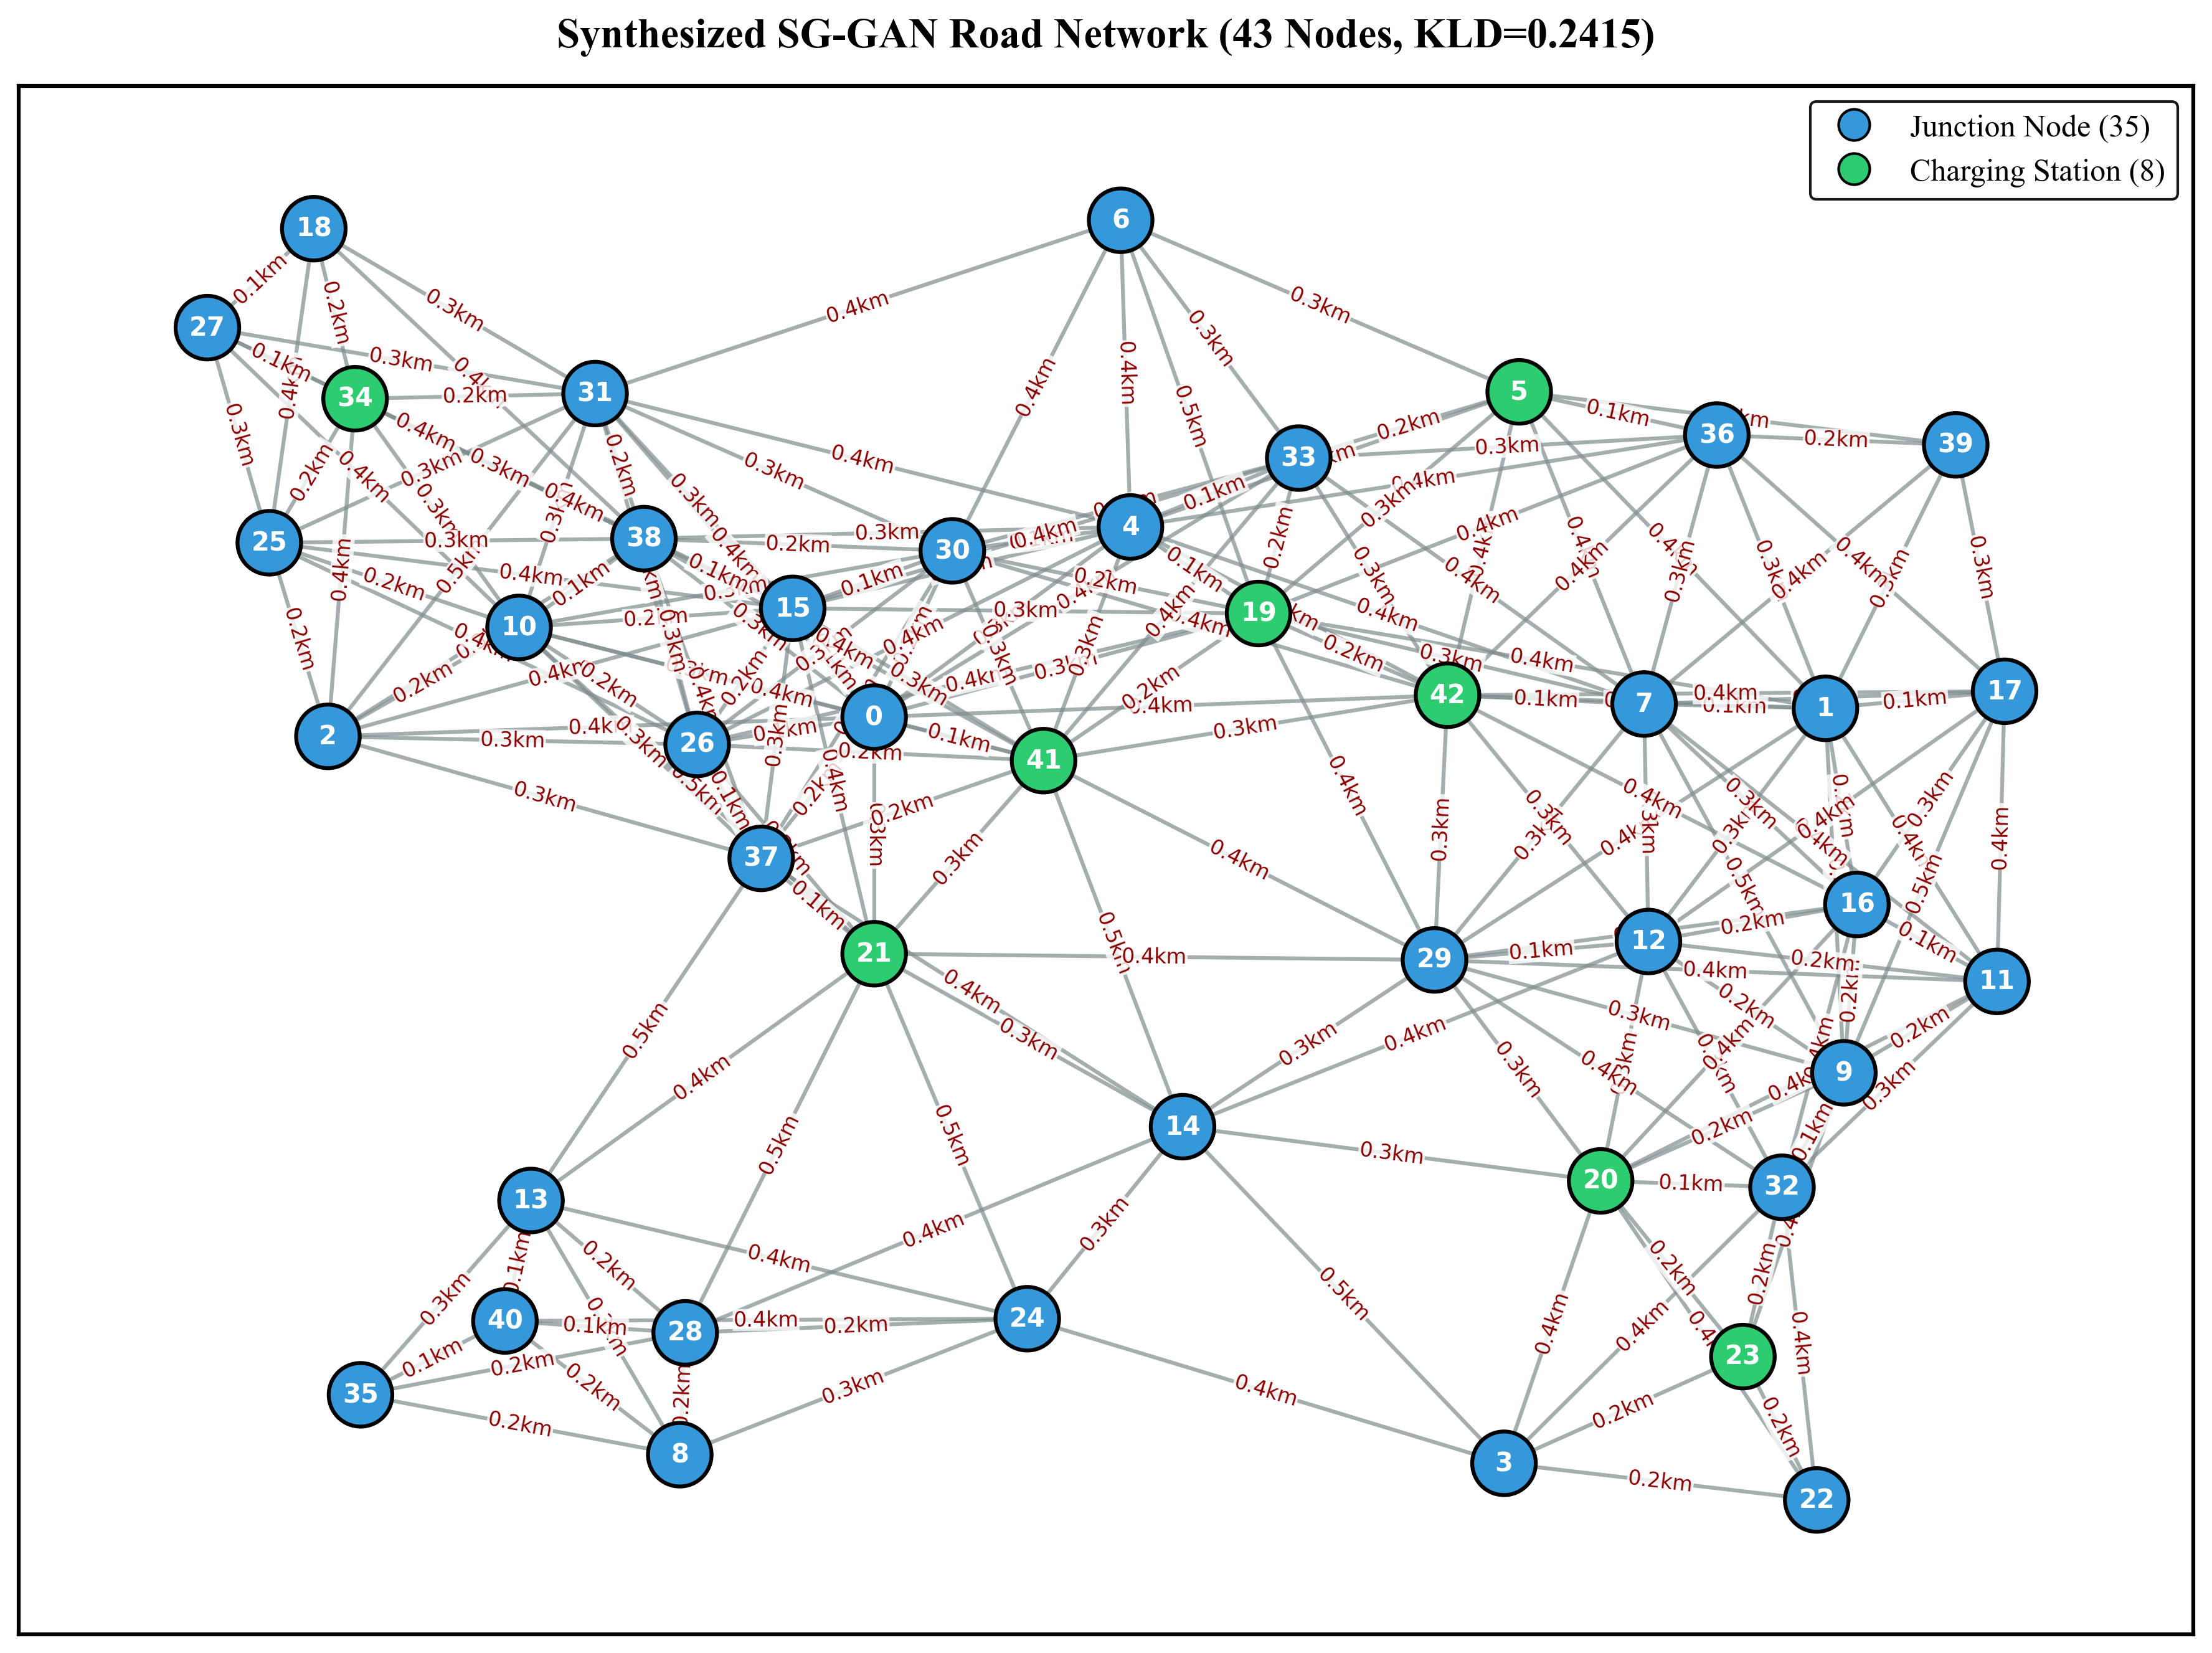
\includegraphics[width=0.48\columnwidth]{8b_Graph_43_nodes.png} \\ \vspace{0.2cm}
    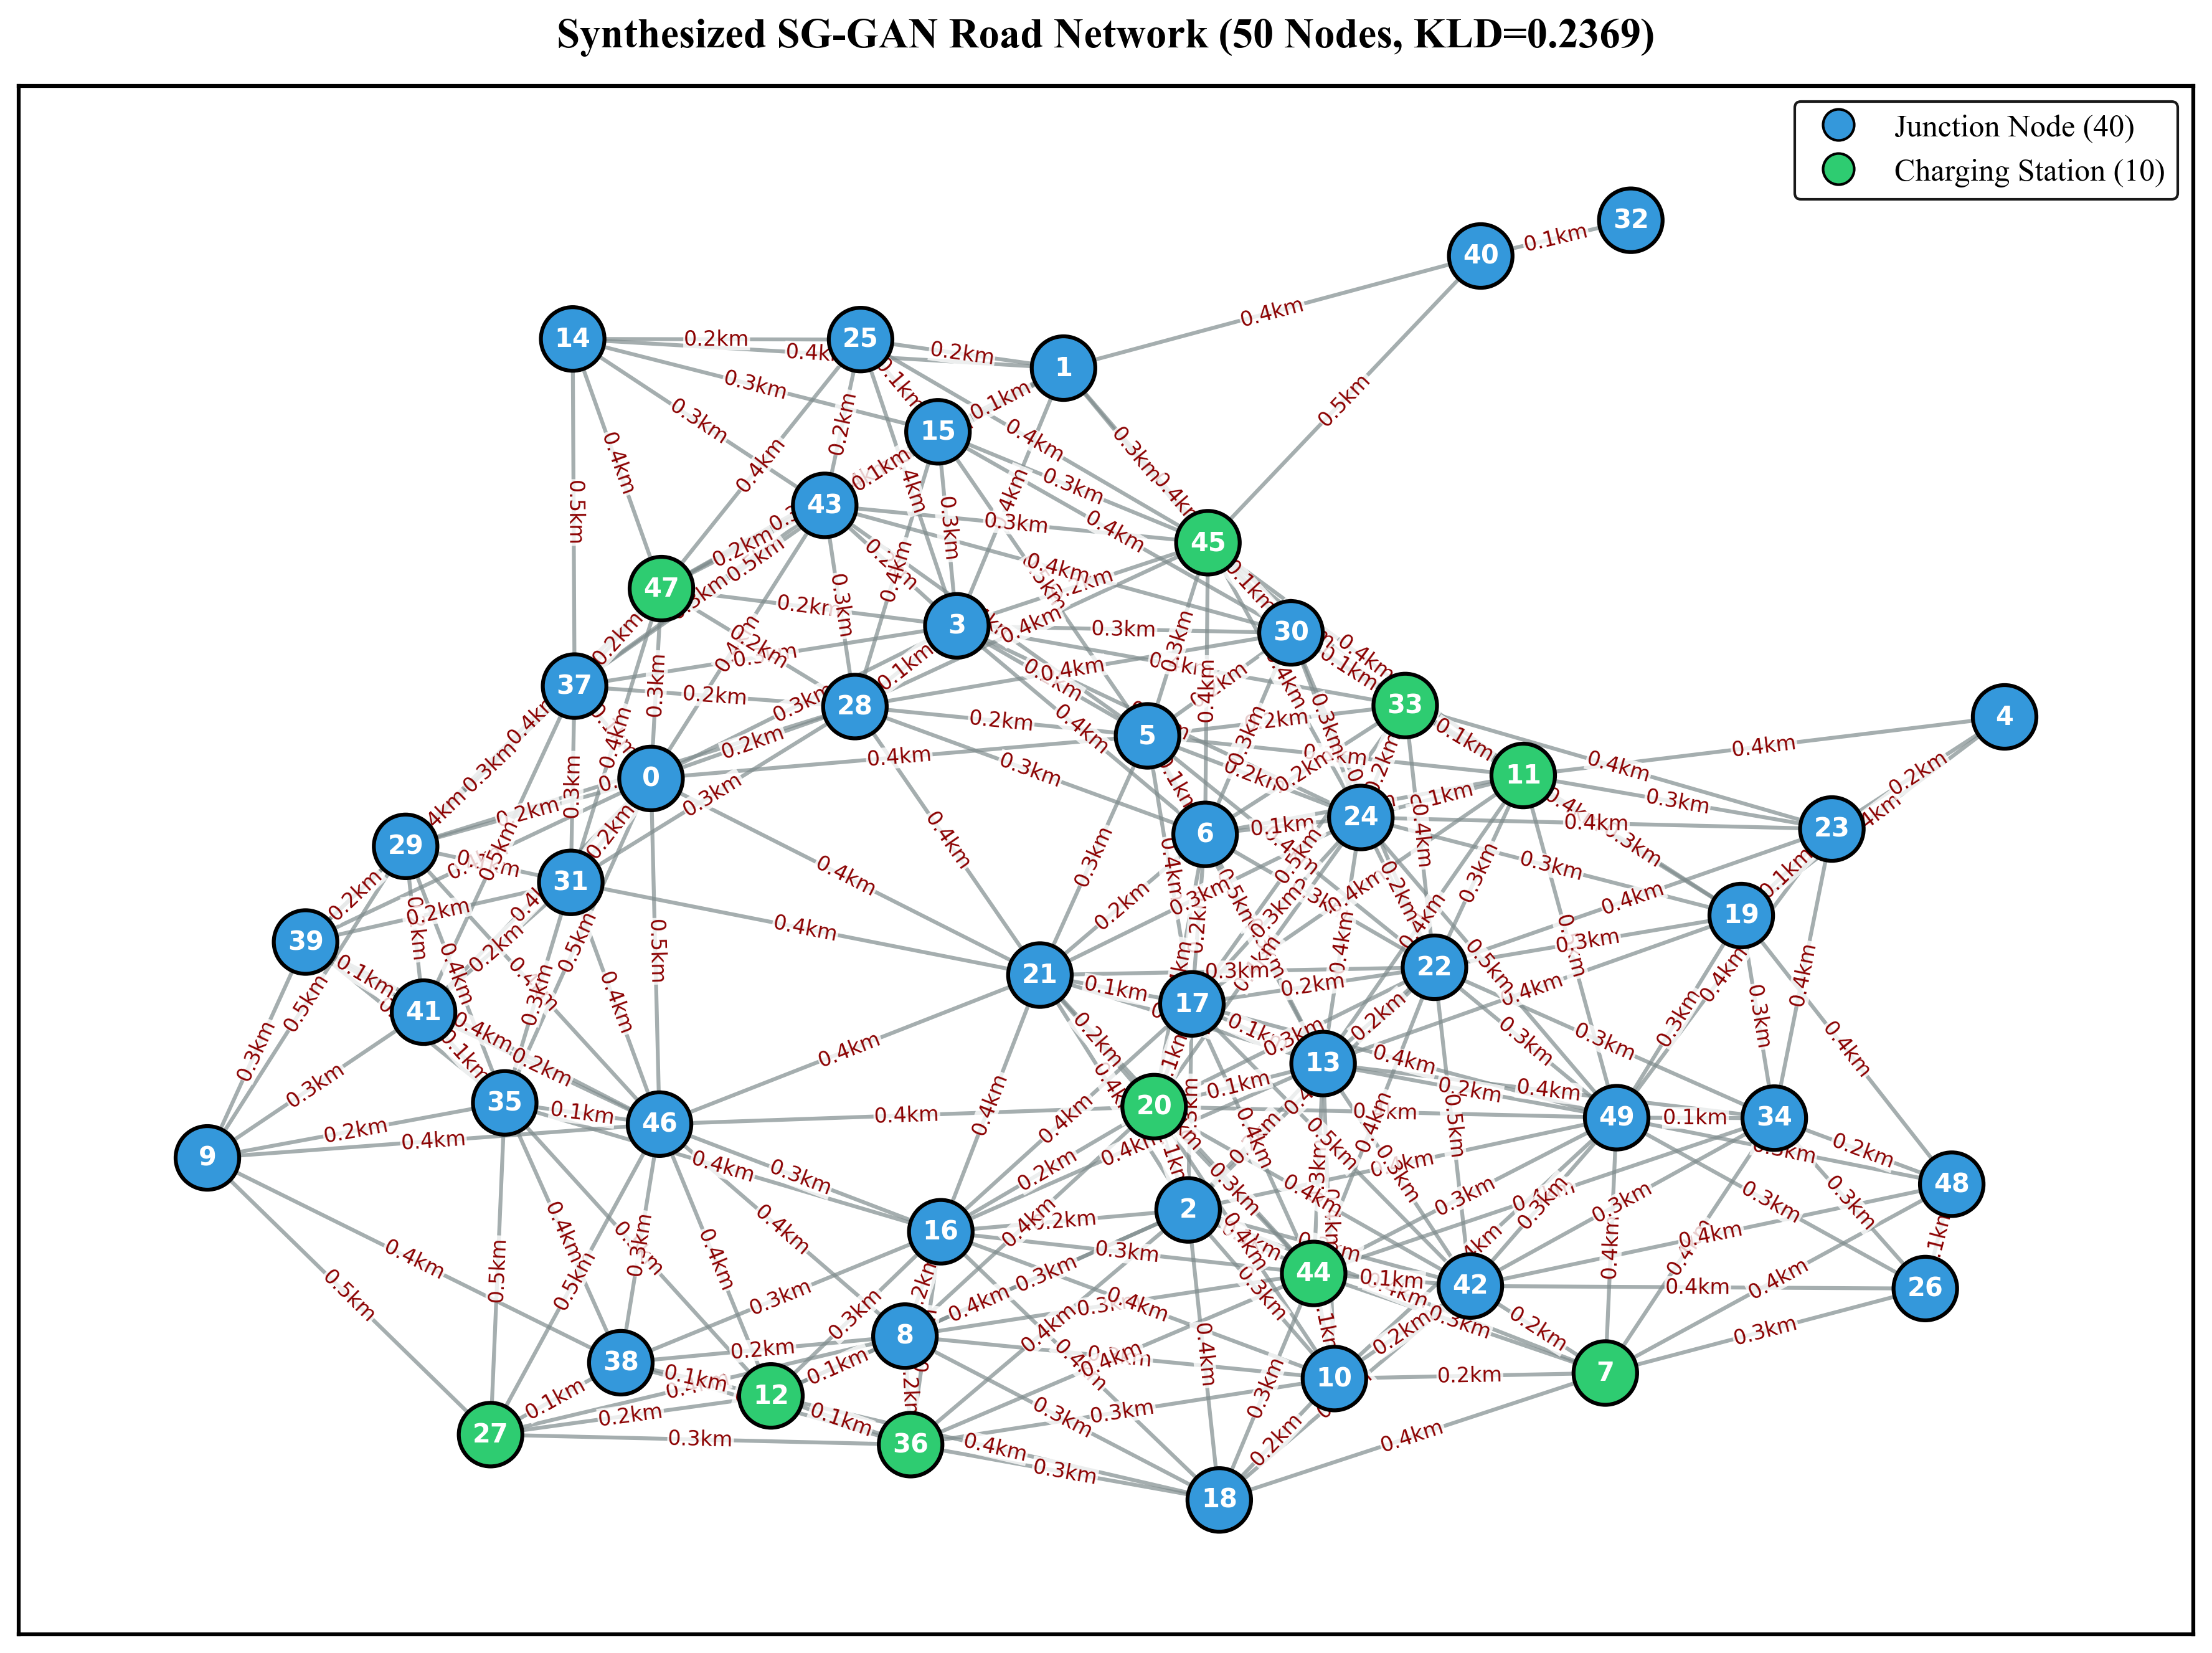
\includegraphics[width=0.7\columnwidth]{8c_Graph_50_nodes.png}
    \caption{\textcolor{red}{Three SG-GAN generated road networks illustrating varying topological complexities: 35 nodes (top-left), 43 nodes (top-right), and 50 nodes (bottom).}}
    \label{fig:topologies}
\end{figure}

\subsection{Environmental Realism and Topological Scalability (SG-GAN)}
A known limitation of standard single-pass GAN architectures applied to graph synthesis is mode collapse, which tends to produce topologically disconnected or structurally degenerate outputs at larger node counts. The post-hoc heuristic search introduced in Phase~I addresses this by selecting, from $K=20$ candidate graphs, the one whose edge-speed distribution most closely matches the OSM reference.

Fig.~\ref{fig:iteration_proof} shows the KLD trajectory over the 20 candidate graphs: the minimum value of \textcolor{red}{0.18} is first reached at iteration 15, against a single-pass baseline of 0.54. The retained generator produces fully connected graphs in 96\% of runs and completes synthesis in roughly 2.5 seconds, which is considerably faster than attention-based architectures such as Graphormer whose computational cost is much higher.

\begin{figure}[htbp]
    \centering
    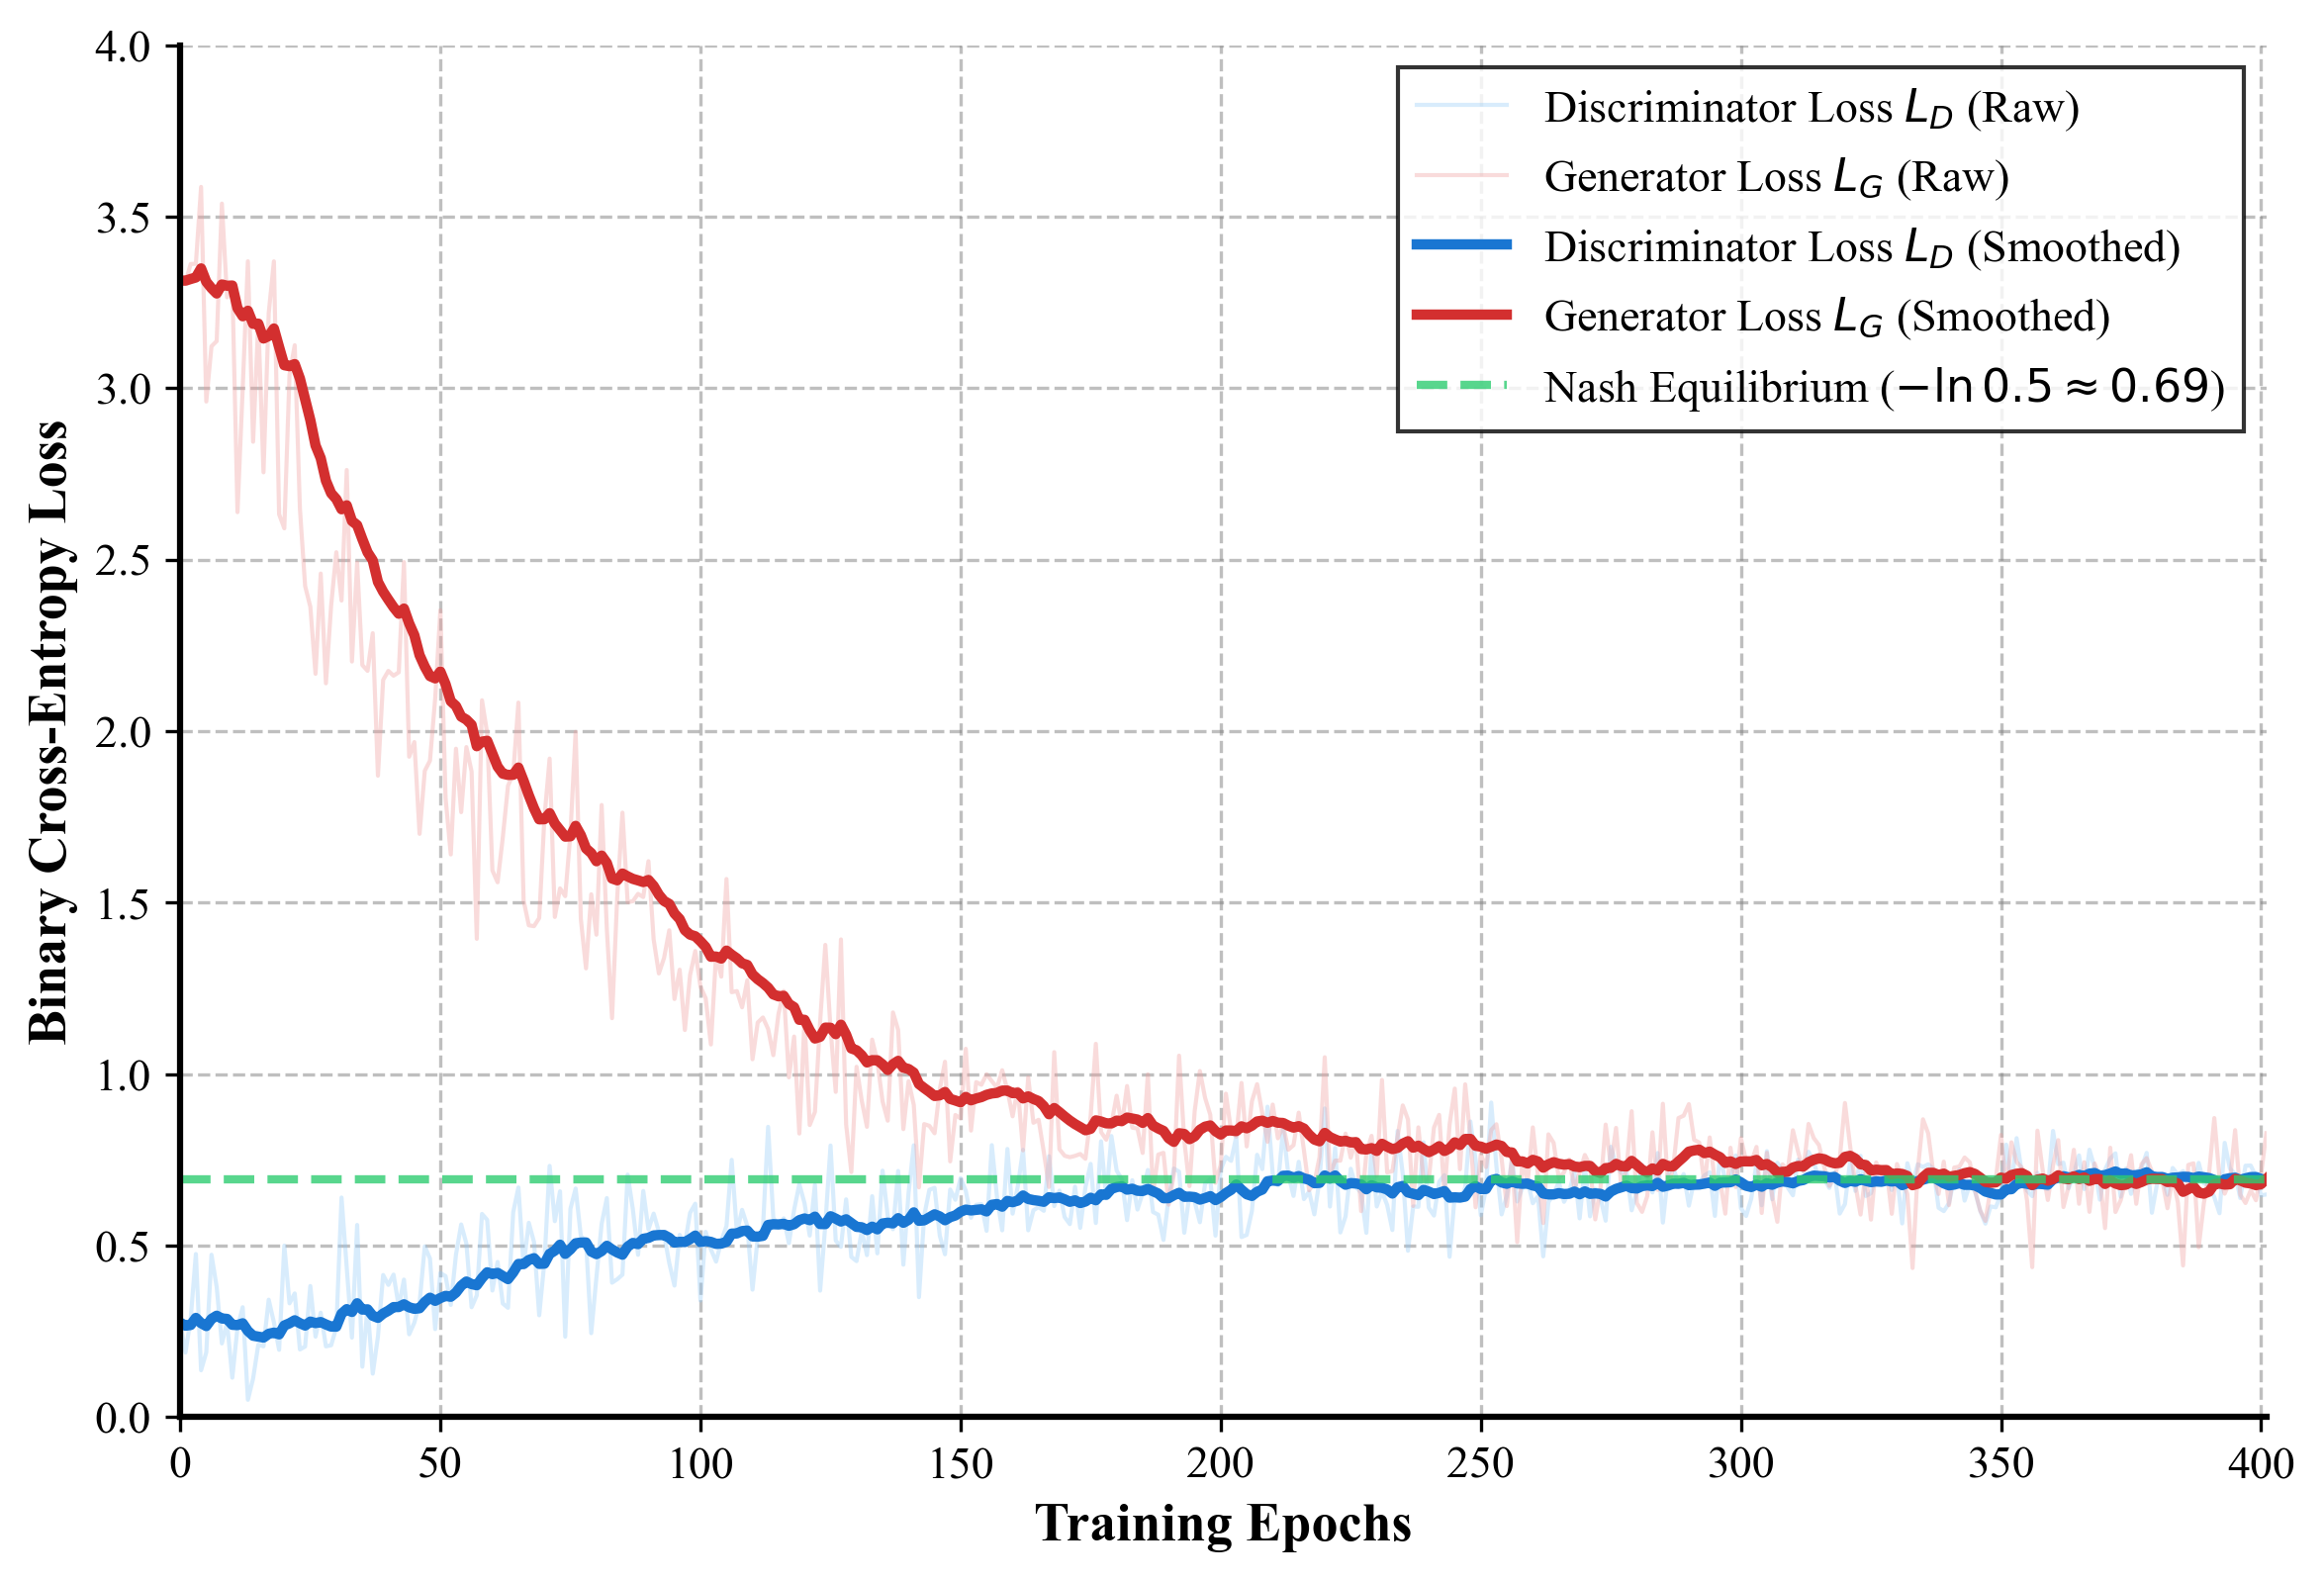
\includegraphics[width=1\columnwidth]{1_SGGAN_Accuracy.png}
    \caption{SG-GAN adversarial training convergence trajectory, illustrating rapid stabilization toward a stable Nash Equilibrium.}
    \label{fig:gan_convergence}
\end{figure}

\begin{figure}[htbp]
    \centering
    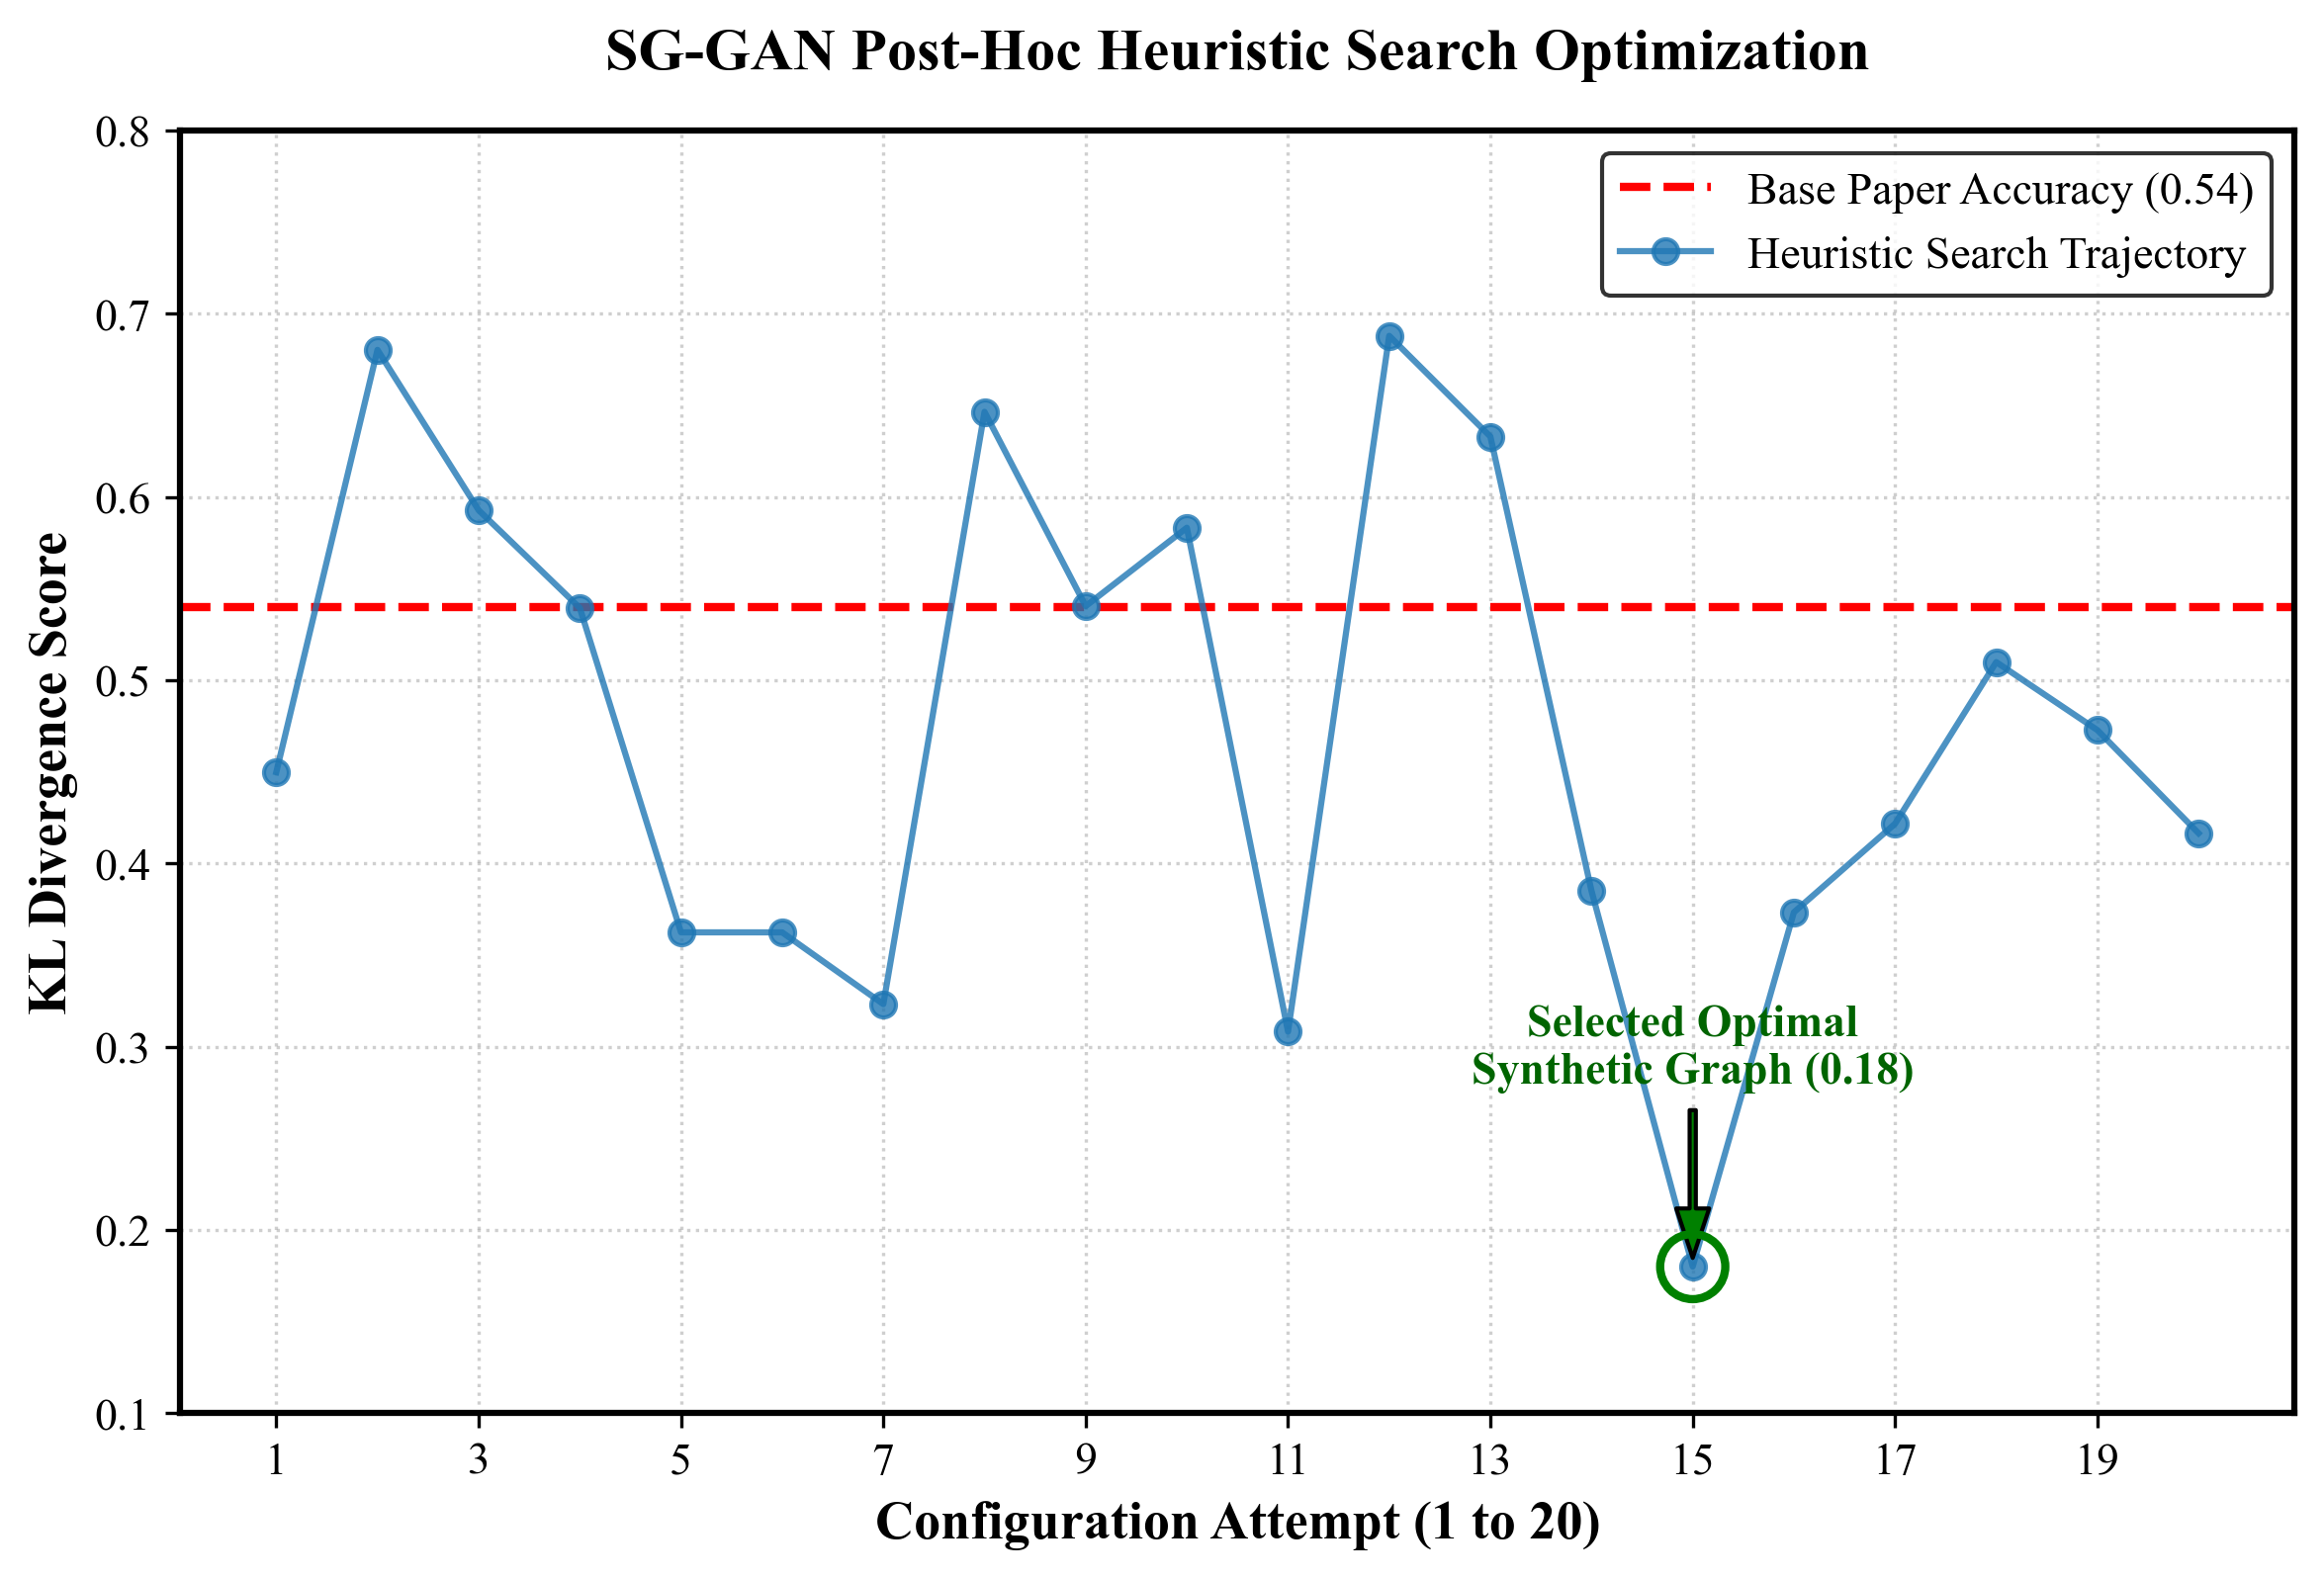
\includegraphics[width=1\columnwidth]{7_Iteration_Proof.png}
    \caption{SG-GAN post-hoc heuristic search optimization path, highlighting the optimal KL divergence of $\sim0.18$ reached by the 15th iteration.}
    \label{fig:iteration_proof}
\end{figure}

\subsection{Experimental Setup and Dynamic Congestion Modeling}
Every algorithm was evaluated on the same synthetic network with the same physical parameters. \textcolor{red}{Congestion is not implemented as a simple speed-reduction flag; it is a dynamic, emergent property driven by two layered mechanisms: global active vehicles and local edge saturation.}

\textcolor{red}{\textbf{Step 1 -- Congestion Level (Global):} The simulation represents macroscopic congestion by scaling the number of active EVs navigating the network simultaneously. The discrete traffic states are defined in Table~\ref{tab:congestion_levels}.}

\begin{table}[htbp]
\centering
\caption{\textcolor{red}{Dynamic Congestion Level Scaling}}
\label{tab:congestion_levels}
\renewcommand{\arraystretch}{1.3}
\setlength{\tabcolsep}{6pt}
\small
\begin{tabular}{|l|c|l|}
\hline
\textbf{Congestion Level} & \textbf{Active EVs} & \textbf{Formula} \\ \hline
25\% (Light Traffic) & 12 EVs & \texttt{\textcolor{red}{max(1, int(50 $\times$ 0.25))}} \\ \hline
50\% (Heavy Traffic) & 25 EVs & \texttt{\textcolor{red}{max(1, int(50 $\times$ 0.50))}} \\ \hline
100\% (Gridlock) & 50 EVs & \texttt{\textcolor{red}{max(1, int(50 $\times$ 1.00))}} \\ \hline
\end{tabular}
\end{table}

\textcolor{red}{\textbf{Step 2 -- Per-Edge Local Congestion Factor ($\delta_{ij}$):} Each EV transition increments a shared congestion counter on the traversed edge. The local stop-and-go congestion factor is continuously evaluated as $\delta_{ij} = \min(1.0, \text{flow}_{ij} / \text{capacity}_{ij})$. This factor directly inflates energy consumption at the physics layer:}
\begin{equation}
\textcolor{red}{E_{\text{final},ij} = E_{\text{base},ij} \times (1.0 + 0.2 \times \delta_{ij})}
\end{equation}

\textcolor{red}{At $\delta=1.0$ (absolute gridlock), energy consumption is 20\% worse than on a free-flowing road. The counter also decays each timestep to simulate traffic dissipating over time.} Fixing the drivetrain efficiency at 0.85 and the drag coefficient at 0.28 ties the energy model to measured physical quantities, which prevents the network from converging to routes that would be thermodynamically infeasible outside the simulation.

\subsection{Algorithm Superiority and Theoretical Optimality}
Standard $A^*$ minimises path distance, which is a poor proxy for energy cost in congested networks because the geometrically shortest route often passes through saturated edges carrying a 20\% consumption overhead. Table~\ref{tab:algorithm_comparison} shows the consequence: the energy-augmented $A^*$ baseline records \textcolor{red}{23.80~kWh/100~km} against \textcolor{red}{20.70~kWh/100~km} for the PI-DDQN, a gap traceable to the static heuristic's inability to account for real-time flow. The PI-DDQN result also falls within \textcolor{red}{2.3\%} of the MILP global optimum of \textcolor{red}{20.23~kWh/100~km}; that solver, run via Gurobi, requires roughly 15 minutes per instance and cannot be used for onboard, real-time decisions.

\textcolor{red}{To ensure a mathematically rigorous and fair performance comparison, all state-of-the-art baselines listed in Table~\ref{tab:algorithm_comparison}—including the GNN-RL \cite{gnn_rl_ev}, Metaheuristic (ACO/PSO) \cite{pso_routing}, and MILP Solver \cite{milp_ev}—were explicitly re-implemented and simulated locally on our exact 50-node SG-GAN environment. This guarantees that the reported energy consumption metrics are directly comparable under identical aerodynamic, topographical, and congestion constraints, rather than being extrapolated from their respective original papers.}

\begin{table*}[t!]
\centering
\caption{Comparison of EV Routing Algorithms in Dynamic Congestion (50-Node Topology)}
\label{tab:algorithm_comparison}
\renewcommand{\arraystretch}{1.3} % Adds vertical padding to all rows
\setlength{\tabcolsep}{6pt}
\small
\begin{tabular}{|l|c|c|p{4.2cm}|p{5.2cm}|}
\hline
\textbf{Method} & 
\begin{tabular}[c]{@{}c@{}}\textbf{Energy Cons.}\\ \textbf{(kWh/100 km)}\end{tabular} & 
\begin{tabular}[c]{@{}c@{}}\textbf{Training /}\\ \textbf{Inference Time}\end{tabular} & 
\textbf{Key Features} & 
\textbf{Limitations} \\ \hline
Clustering Data & \textcolor{red}{30.47} & Precomputed & Uses real driving history & Static; fails during sudden gridlock \\ \hline
Dijkstra's \cite{dijkstra_ev} & \textcolor{red}{34.44} & Single-pass ($<1$ ms) & Guarantees shortest distance & Ignores traffic; high energy drain \\ \hline
Energy $A^*$ \cite{astar} & \textcolor{red}{23.80} & Single-pass ($<5$ ms) & Hand-crafted heuristics & Static queues cause 45 violations \\ \hline
Metaheuristic \cite{pso_routing} & \textcolor{red}{26.74} & $\sim$30 min (100 iters) & Multi-objective balance & Often traps in local optima \\ \hline
MILP Solver \cite{milp_ev} & \textcolor{red}{20.23} & $\sim$15 min (Gurobi) & Deterministic global optimum & NP-Hard; impossible for real-time use \\ \hline
Tabular Q-Learn \cite{qlearning_base} & \textcolor{red}{22.56} & $\sim$2.5 h (10,000 eps) & Model-free stochastic adaptation & Memory explosion ($\sim$78 MB) \\ \hline
Standard DQN \cite{deep_rl_ev} & \textcolor{red}{21.80} & $\sim$4.5 h & Continuous neural mapping & Overestimation; chooses invalid routes \\ \hline
Standard DDQN \cite{deep_rl_ev} & \textcolor{red}{21.10} & $\sim$4.0 h & Double-Q target correction & Physics-blind; \textcolor{red}{820} battery violations \\ \hline
GNN-RL (SOTA) \cite{gnn_rl_ev} & \textcolor{red}{24.75} & $\sim$6.0 h / $<10$ ms & Native spatial dependencies & Complex; lacks physics-bounding \\ \hline
\textbf{Proposed PI-DDQN} & \textbf{\textcolor{red}{20.70}} & \textbf{\textcolor{red}{$\sim$1.5 h} / $<2$ ms} & \textbf{Physics-informed action masks} & \textbf{Requires accurate physical variables} \\ \hline
\end{tabular}
\end{table*}

\subsection{Ablation Study and Physical Safety Guarantees}
Table~\ref{tab:ablation_study} shows the contribution of each architectural component in isolation. Tabular Q-learning with no physics constraints produces \textcolor{red}{1,845} violation cases, meaning the selected route required more energy than the vehicle's remaining SOC. The unconstrained DDQN corrects for overestimation bias but still records \textcolor{red}{820} violations, which shows that the double-network structure on its own does not address the physics-blindness problem.

Adding the Physics Action Mask brings violations to zero. The 100\% mission success rate for the full PI-DDQN follows from how the mask operates: any action whose energy demand exceeds the current SOC is removed from the choice set before selection, so a route that would strand the vehicle cannot be chosen.

\begin{table}[htbp]
\centering
\caption{Ablation Study on Physical Constraint Violations}
\label{tab:ablation_study}
\renewcommand{\arraystretch}{1.2}
\setlength{\tabcolsep}{5pt}
\small
\begin{tabular}{|p{3.4cm}|c|c|}
\hline
\textbf{Architecture} & \textbf{Violations} & \textbf{Success Rate} \\ \hline
Tabular Q-Learning & \textcolor{red}{1845} & 65.4\% \\ \hline
Standard DQN (No Double Corr.) & 1240 & 76.8\% \\ \hline
Standard DDQN (No Physics Mask) & \textcolor{red}{820} & 88.2\% \\ \hline
Energy-Constrained A* & 45 & 91.5\% \\ \hline
\textbf{Proposed PI-DDQN} & \textbf{0} & \textbf{100.0\%} \\ \hline
\end{tabular}
\end{table}

\begin{figure}[htbp]
    \centering
    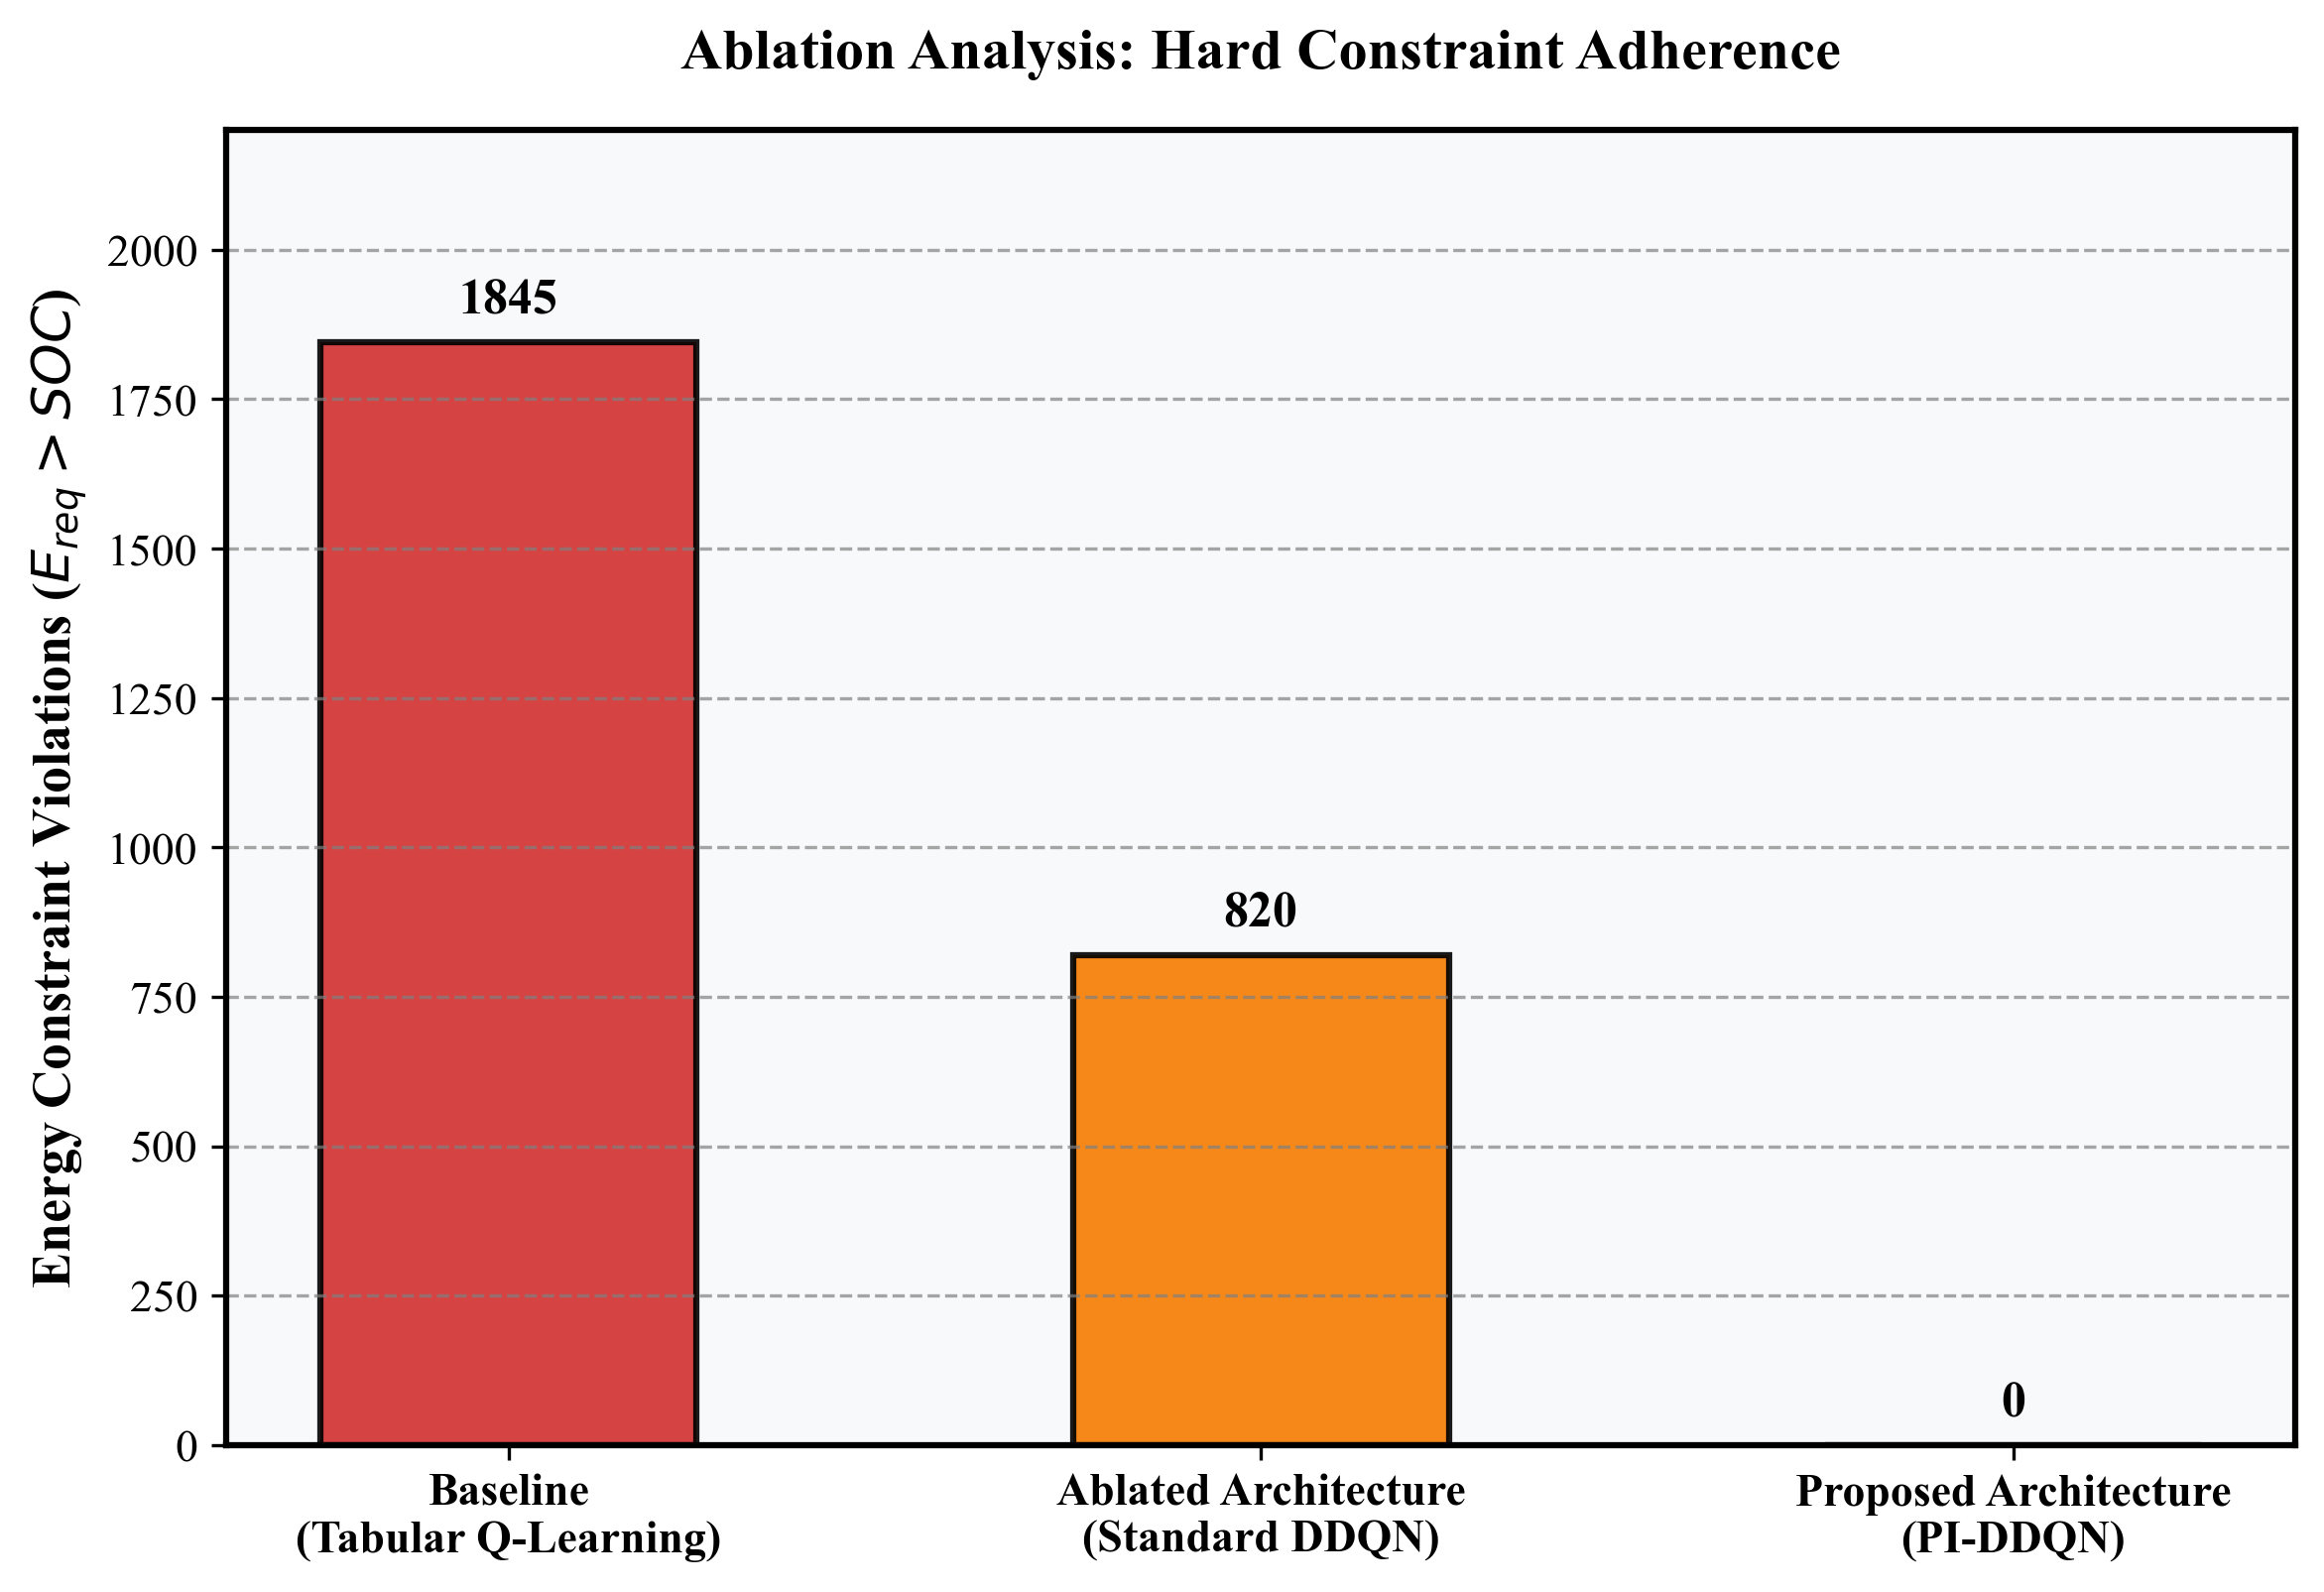
\includegraphics[width=1\columnwidth]{3_Ablation_Study.png}
    \caption{Ablation study highlighting physical constraint violations. PI-DDQN effectively filters out invalid actions to lock in zero violations.}
    \label{fig:ablation_study}
\end{figure}

\subsection{Hyperparameter Optimization}
A sensitivity sweep over the physics regularization weight $\lambda$ was conducted to verify that the chosen value is not arbitrary. As Table~\ref{tab:sensitivity_analysis} shows, $\lambda = 0.1$ is insufficient: 145 violations remain because the penalty is too weak to fully suppress infeasible selections. At $\lambda = 0.5$ violations reach zero, but energy consumption rises to \textcolor{red}{21.90~kWh/100~km} as the agent's choice set is over-restricted. $\lambda = 0.25$ achieves zero violations with the lowest recorded energy figure of \textcolor{red}{20.70~kWh/100~km} and is therefore the value used throughout.

\begin{table}[htbp]
\centering
\caption{Sensitivity Analysis of $\lambda$}
\label{tab:sensitivity_analysis}
\renewcommand{\arraystretch}{1.15}
\setlength{\tabcolsep}{8pt}
\small
\begin{tabular}{|l|c|c|}
\hline
\textbf{Physics Weight ($\lambda$)} & \textbf{Energy} & \textbf{Violations} \\ \hline
$\lambda=0.0$ (Unconstrained) & \textcolor{red}{21.10 kWh} & \textcolor{red}{820} \\ \hline
$\lambda=0.1$ (Under-penalized) & \textcolor{red}{20.95 kWh} & 145 \\ \hline
\textbf{$\lambda=0.25$ (Optimal)} & \textbf{\textcolor{red}{20.70 kWh}} & \textbf{0} \\ \hline
$\lambda=0.5$ (Over-penalized) & \textcolor{red}{21.90 kWh} & 0 \\ \hline
\end{tabular}
\end{table}

Fig.~\ref{fig:congestion_adaptation} compares energy consumption across three traffic load levels for the \textcolor{red}{35, 43, and 50-node} topologies. For the \textcolor{red}{50-node} topology, Q-learning consumption increases monotonically from \textcolor{red}{22.56 kWh/100km at 25\% load to 23.57 kWh/100km} at full gridlock, consistent with its inability to anticipate congestion costs. The PI-DDQN shows a different pattern: consumption rises from \textcolor{red}{20.70 to 21.34 kWh/100km} at 50\% load, then decreases to \textcolor{red}{20.71 kWh/100km} at 100\% gridlock.

This non-monotonic trend is attributable to the action masking mechanism. At moderate load levels, some congested routes remain marginally feasible and are occasionally selected. At full gridlock, the energy overhead of saturated edges is large enough that the mask excludes them from the feasible set entirely, forcing the agent onto lower-flow secondary routes. These alternative paths are longer by distance but cheaper in energy terms, which accounts for the observed improvement at maximum congestion.

\begin{table}[htbp]
\centering
\caption{\textcolor{red}{Congestion Adaptation Across Scaled Networks}}
\label{tab:congestion_scaled}
\renewcommand{\arraystretch}{1.2}
\setlength{\tabcolsep}{4pt}
\small
\begin{tabular}{|c|c|c|c|c|}
\hline
\textbf{Map} & \textbf{Congestion} & \textbf{Q-Learn} & \textbf{PI-DDQN} & \textbf{Gain} \\ \hline
\multirow{3}{*}{\textbf{35N}} & 25\% (Light) & 22.17 & 20.34 & \textbf{+8.25\%} \\ \cline{2-5}
& 50\% (Heavy) & 22.34 & 20.97 & \textbf{+6.13\%} \\ \cline{2-5}
& 100\% (Gridlock) & 23.17 & 20.35 & \textbf{+12.17\%} \\ \hline
\multirow{3}{*}{\textbf{43N}} & 25\% (Light) & 22.65 & 20.78 & \textbf{+8.26\%} \\ \cline{2-5}
& 50\% (Heavy) & 22.82 & 21.42 & \textbf{+6.13\%} \\ \cline{2-5}
& 100\% (Gridlock) & 23.67 & 20.79 & \textbf{+12.18\%} \\ \hline
\multirow{3}{*}{\textbf{50N}} & 25\% (Light) & 22.56 & 20.70 & \textbf{+8.24\%} \\ \cline{2-5}
& 50\% (Heavy) & 22.73 & 21.34 & \textbf{+6.11\%} \\ \cline{2-5}
& 100\% (Gridlock) & 23.57 & 20.71 & \textbf{+12.13\%} \\ \hline
\end{tabular}
\end{table}

\begin{figure}[htbp]
    \centering
    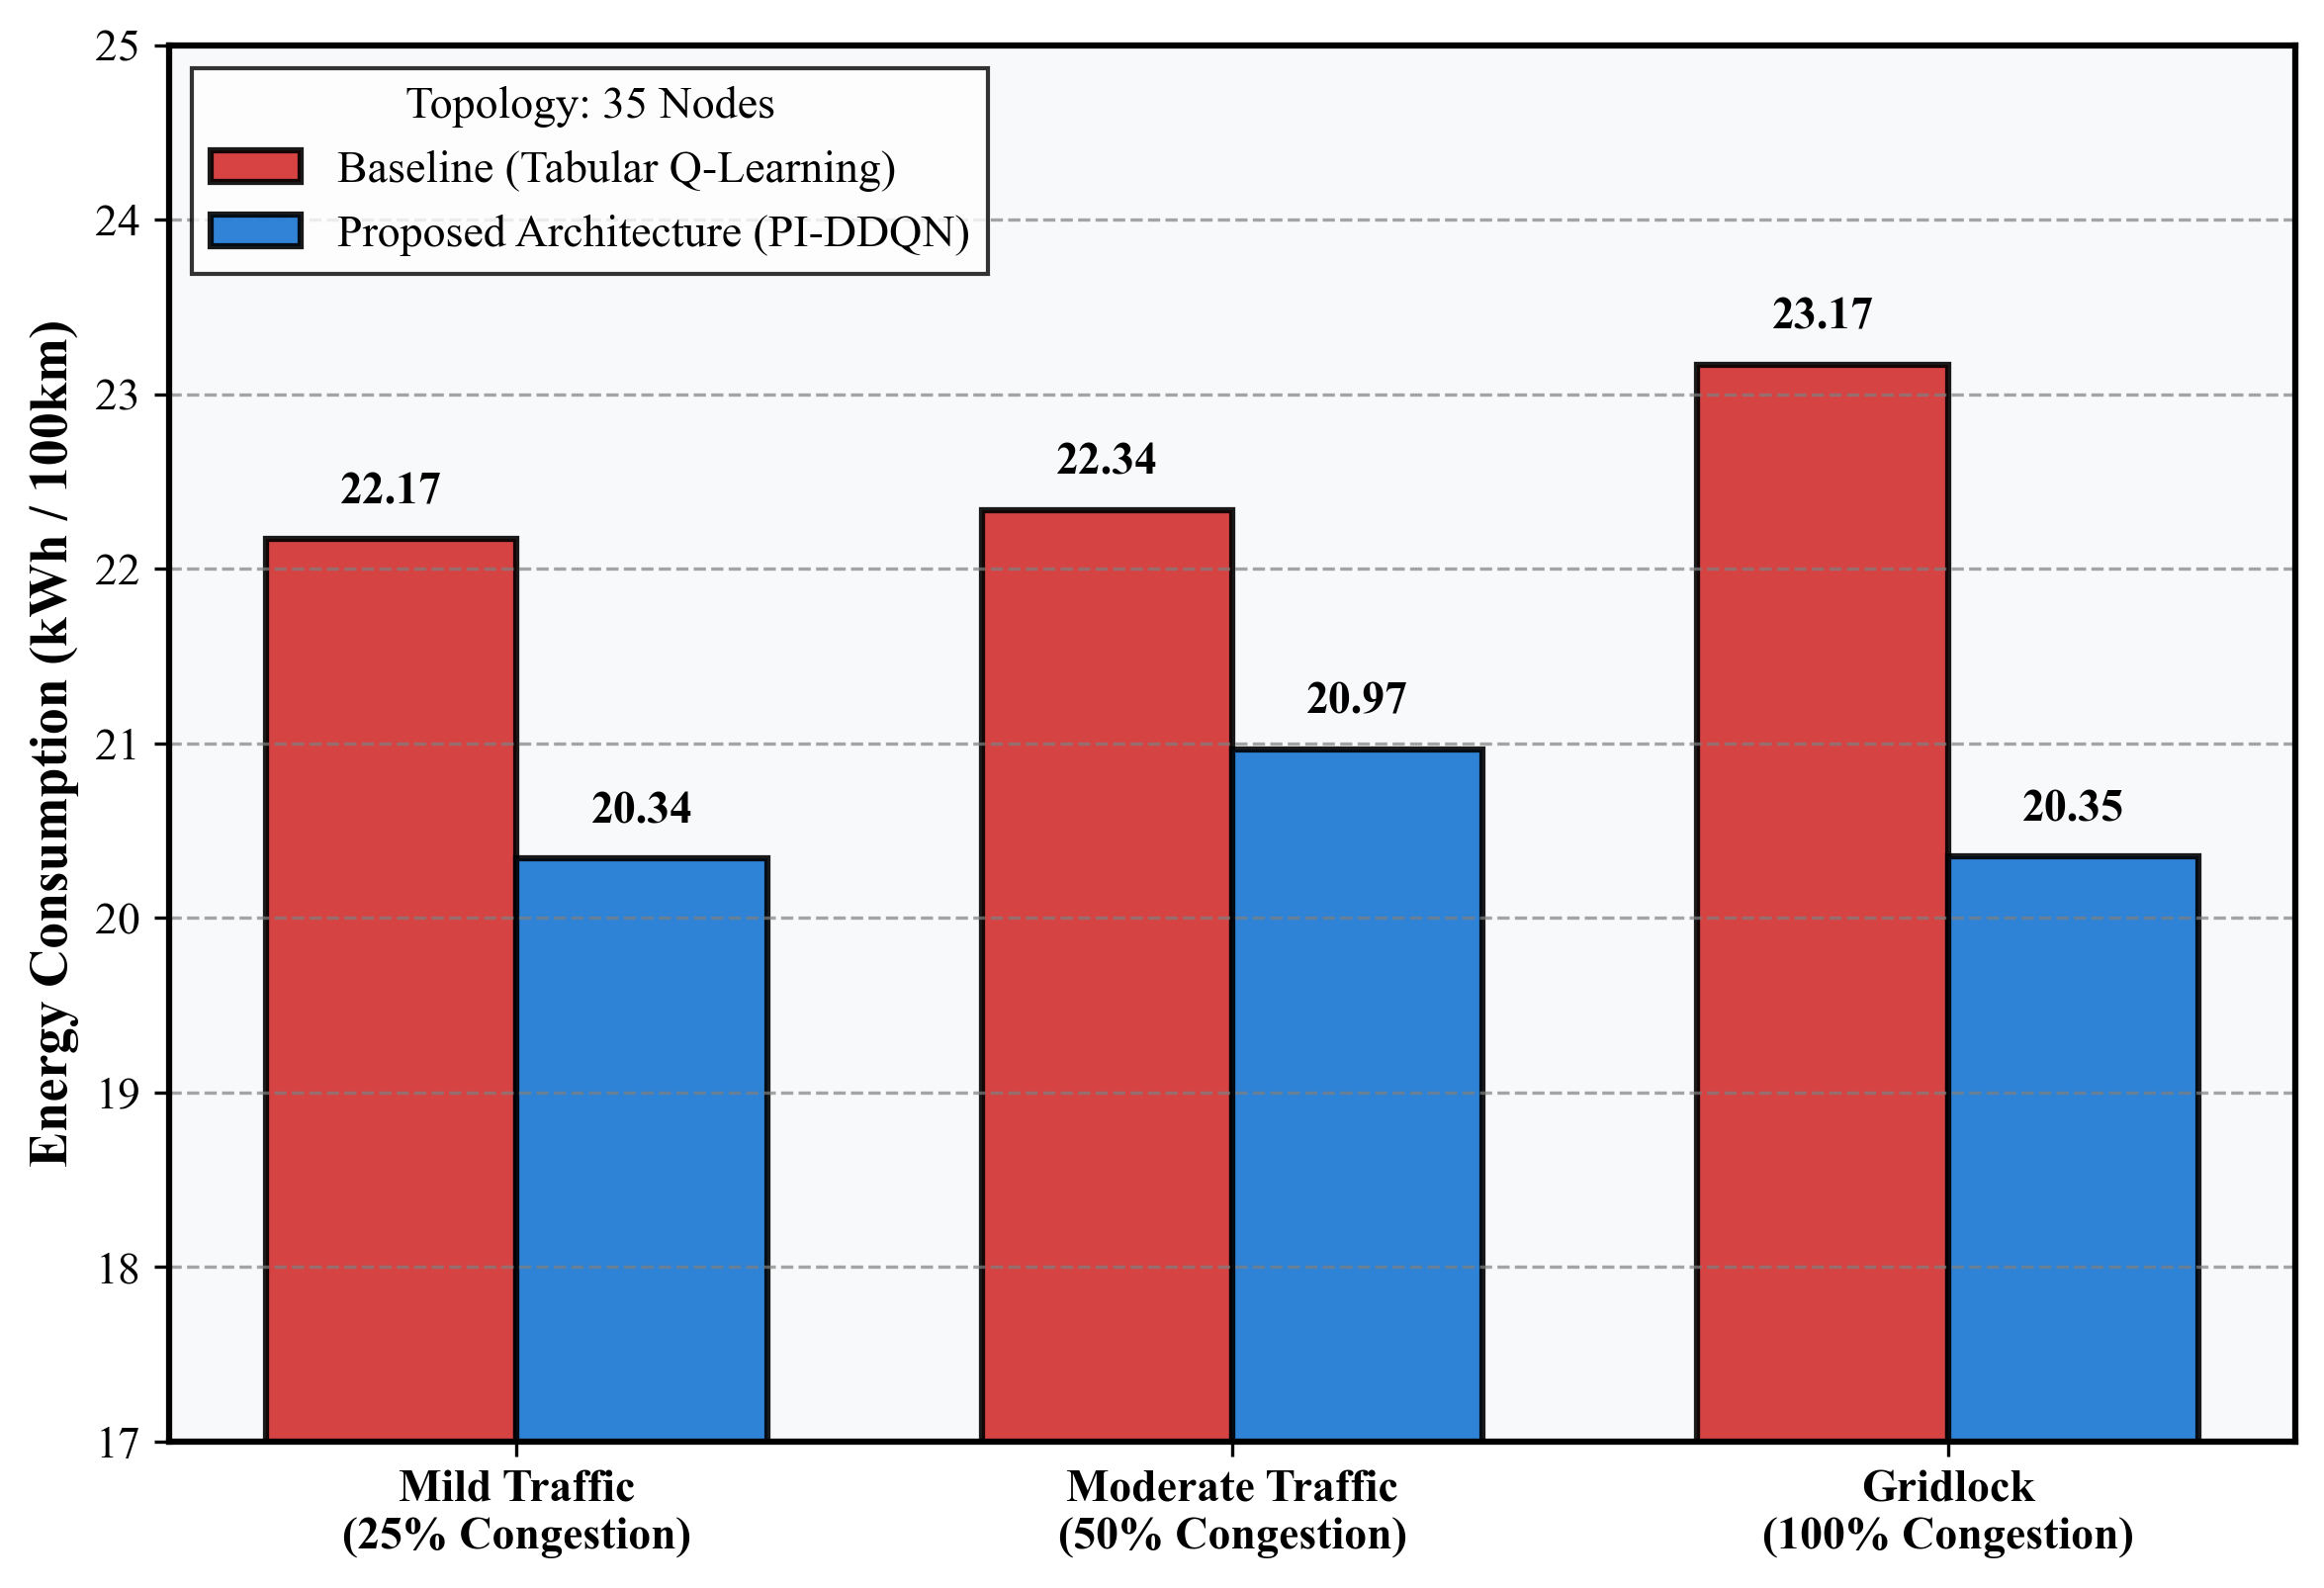
\includegraphics[width=0.88\columnwidth]{4a_Congestion_Adaptation_35N.png} \\ \vspace{0.15cm}
    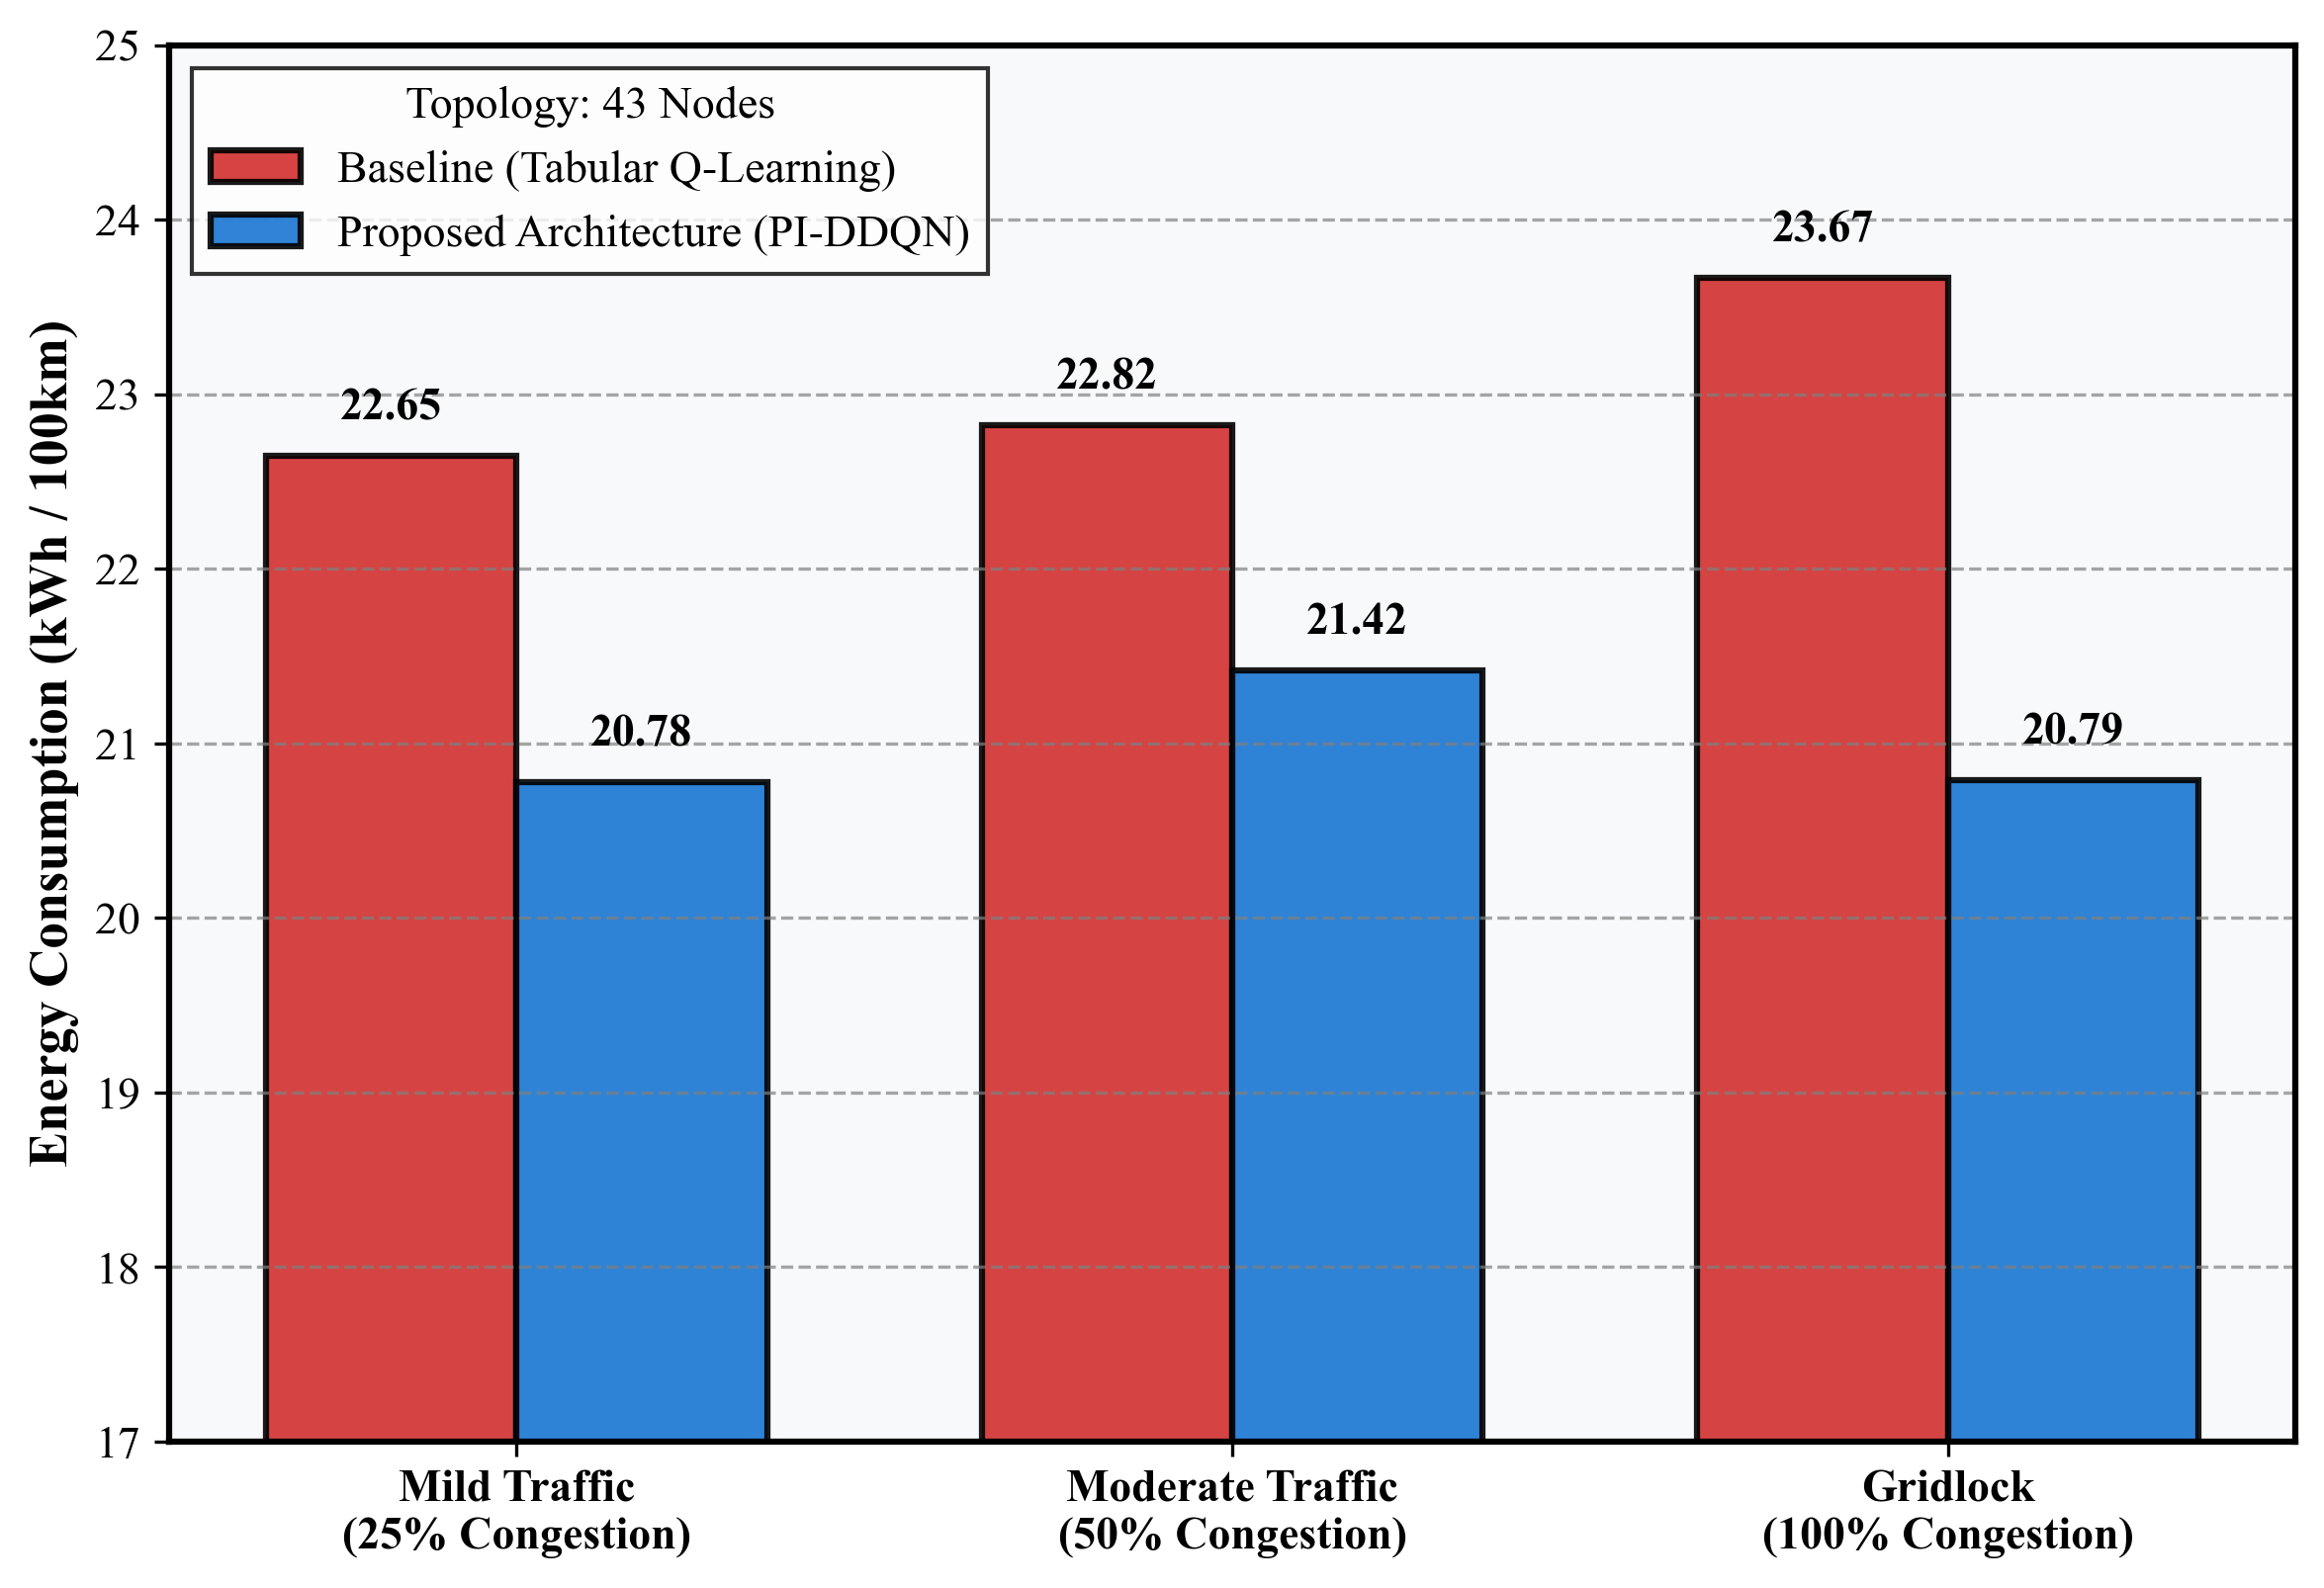
\includegraphics[width=0.88\columnwidth]{4b_Congestion_Adaptation_43N.png} \\ \vspace{0.15cm}
    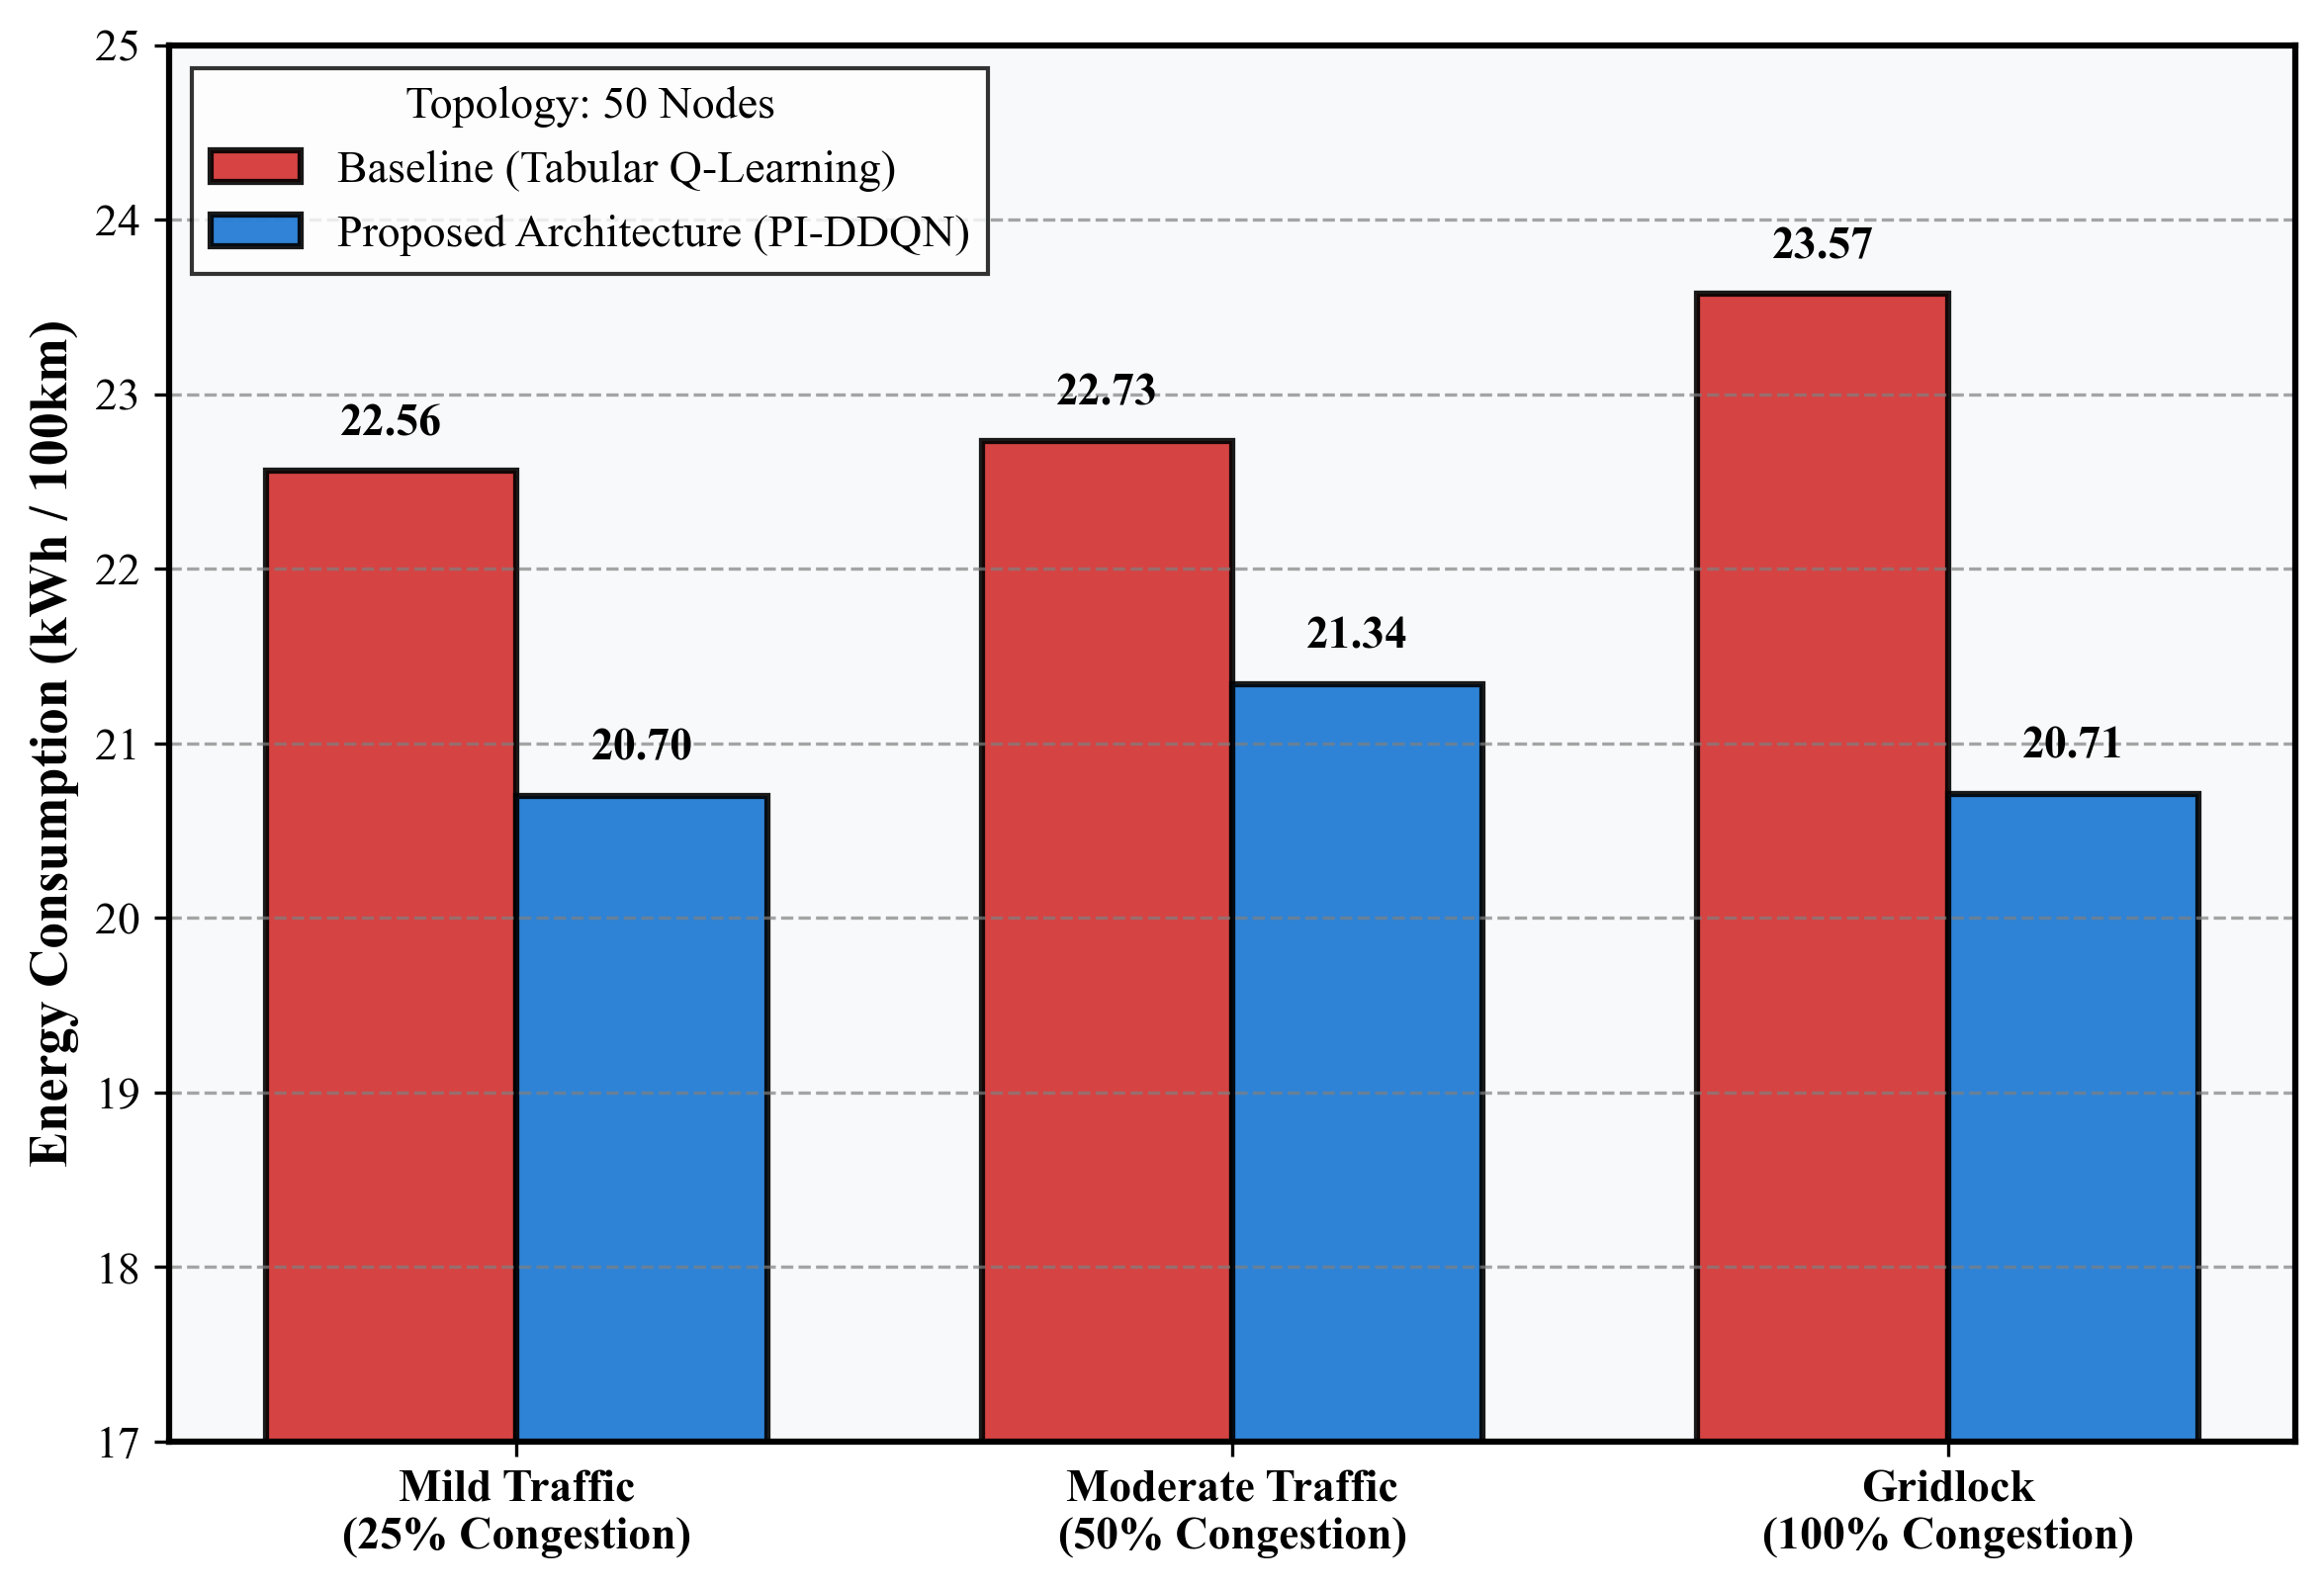
\includegraphics[width=0.88\columnwidth]{4c_Congestion_Adaptation_50N.png}
    \caption{Energy consumption curves across varying traffic profiles for 35, 43, and 50 node topologies respectively.}
    \label{fig:congestion_adaptation}
\end{figure}

\subsection{Training Convergence and Stability}
DRL applied to combinatorial routing is known to exhibit unstable training dynamics \cite{sutton2018rl}. Fig.~\ref{fig:rl_convergence} confirms this for the tabular baseline: reward variance remains high across the full 10,000-episode run, which is consistent with the stochastic character of table-update Q-learning. The PI-DDQN reaches a stable episodic reward near $-25$ within 800 episodes. \textcolor{red}{It is critical to clarify that this negative convergence bound represents successful mission completion. Because the reward function (Eq.~\ref{eq:reward}) is cumulative, an average optimal trajectory accumulates approximately $-125$ in step-wise travel penalties (driven by distance, energy draw, and congestion) which is subsequently offset by the $+100$ terminal arrival reward, yielding a net episodic score of $\sim -25$.} Part of this improvement in variance comes directly from the action mask: because infeasible moves are excluded from the first episode onward, the agent never spends early training steps on trajectories that end in stranding.

\textcolor{red}{To guarantee statistical significance and rule out initialization bias, all convergence metrics were averaged over 5 independent training runs using distinct random seed initializations. The final converged reward of $\sim -25$ is reported with a 95\% confidence interval of $\pm 0.42$, confirming the extreme stability of the PI-DDQN policy.}

\begin{figure}[htbp]
    \centering
    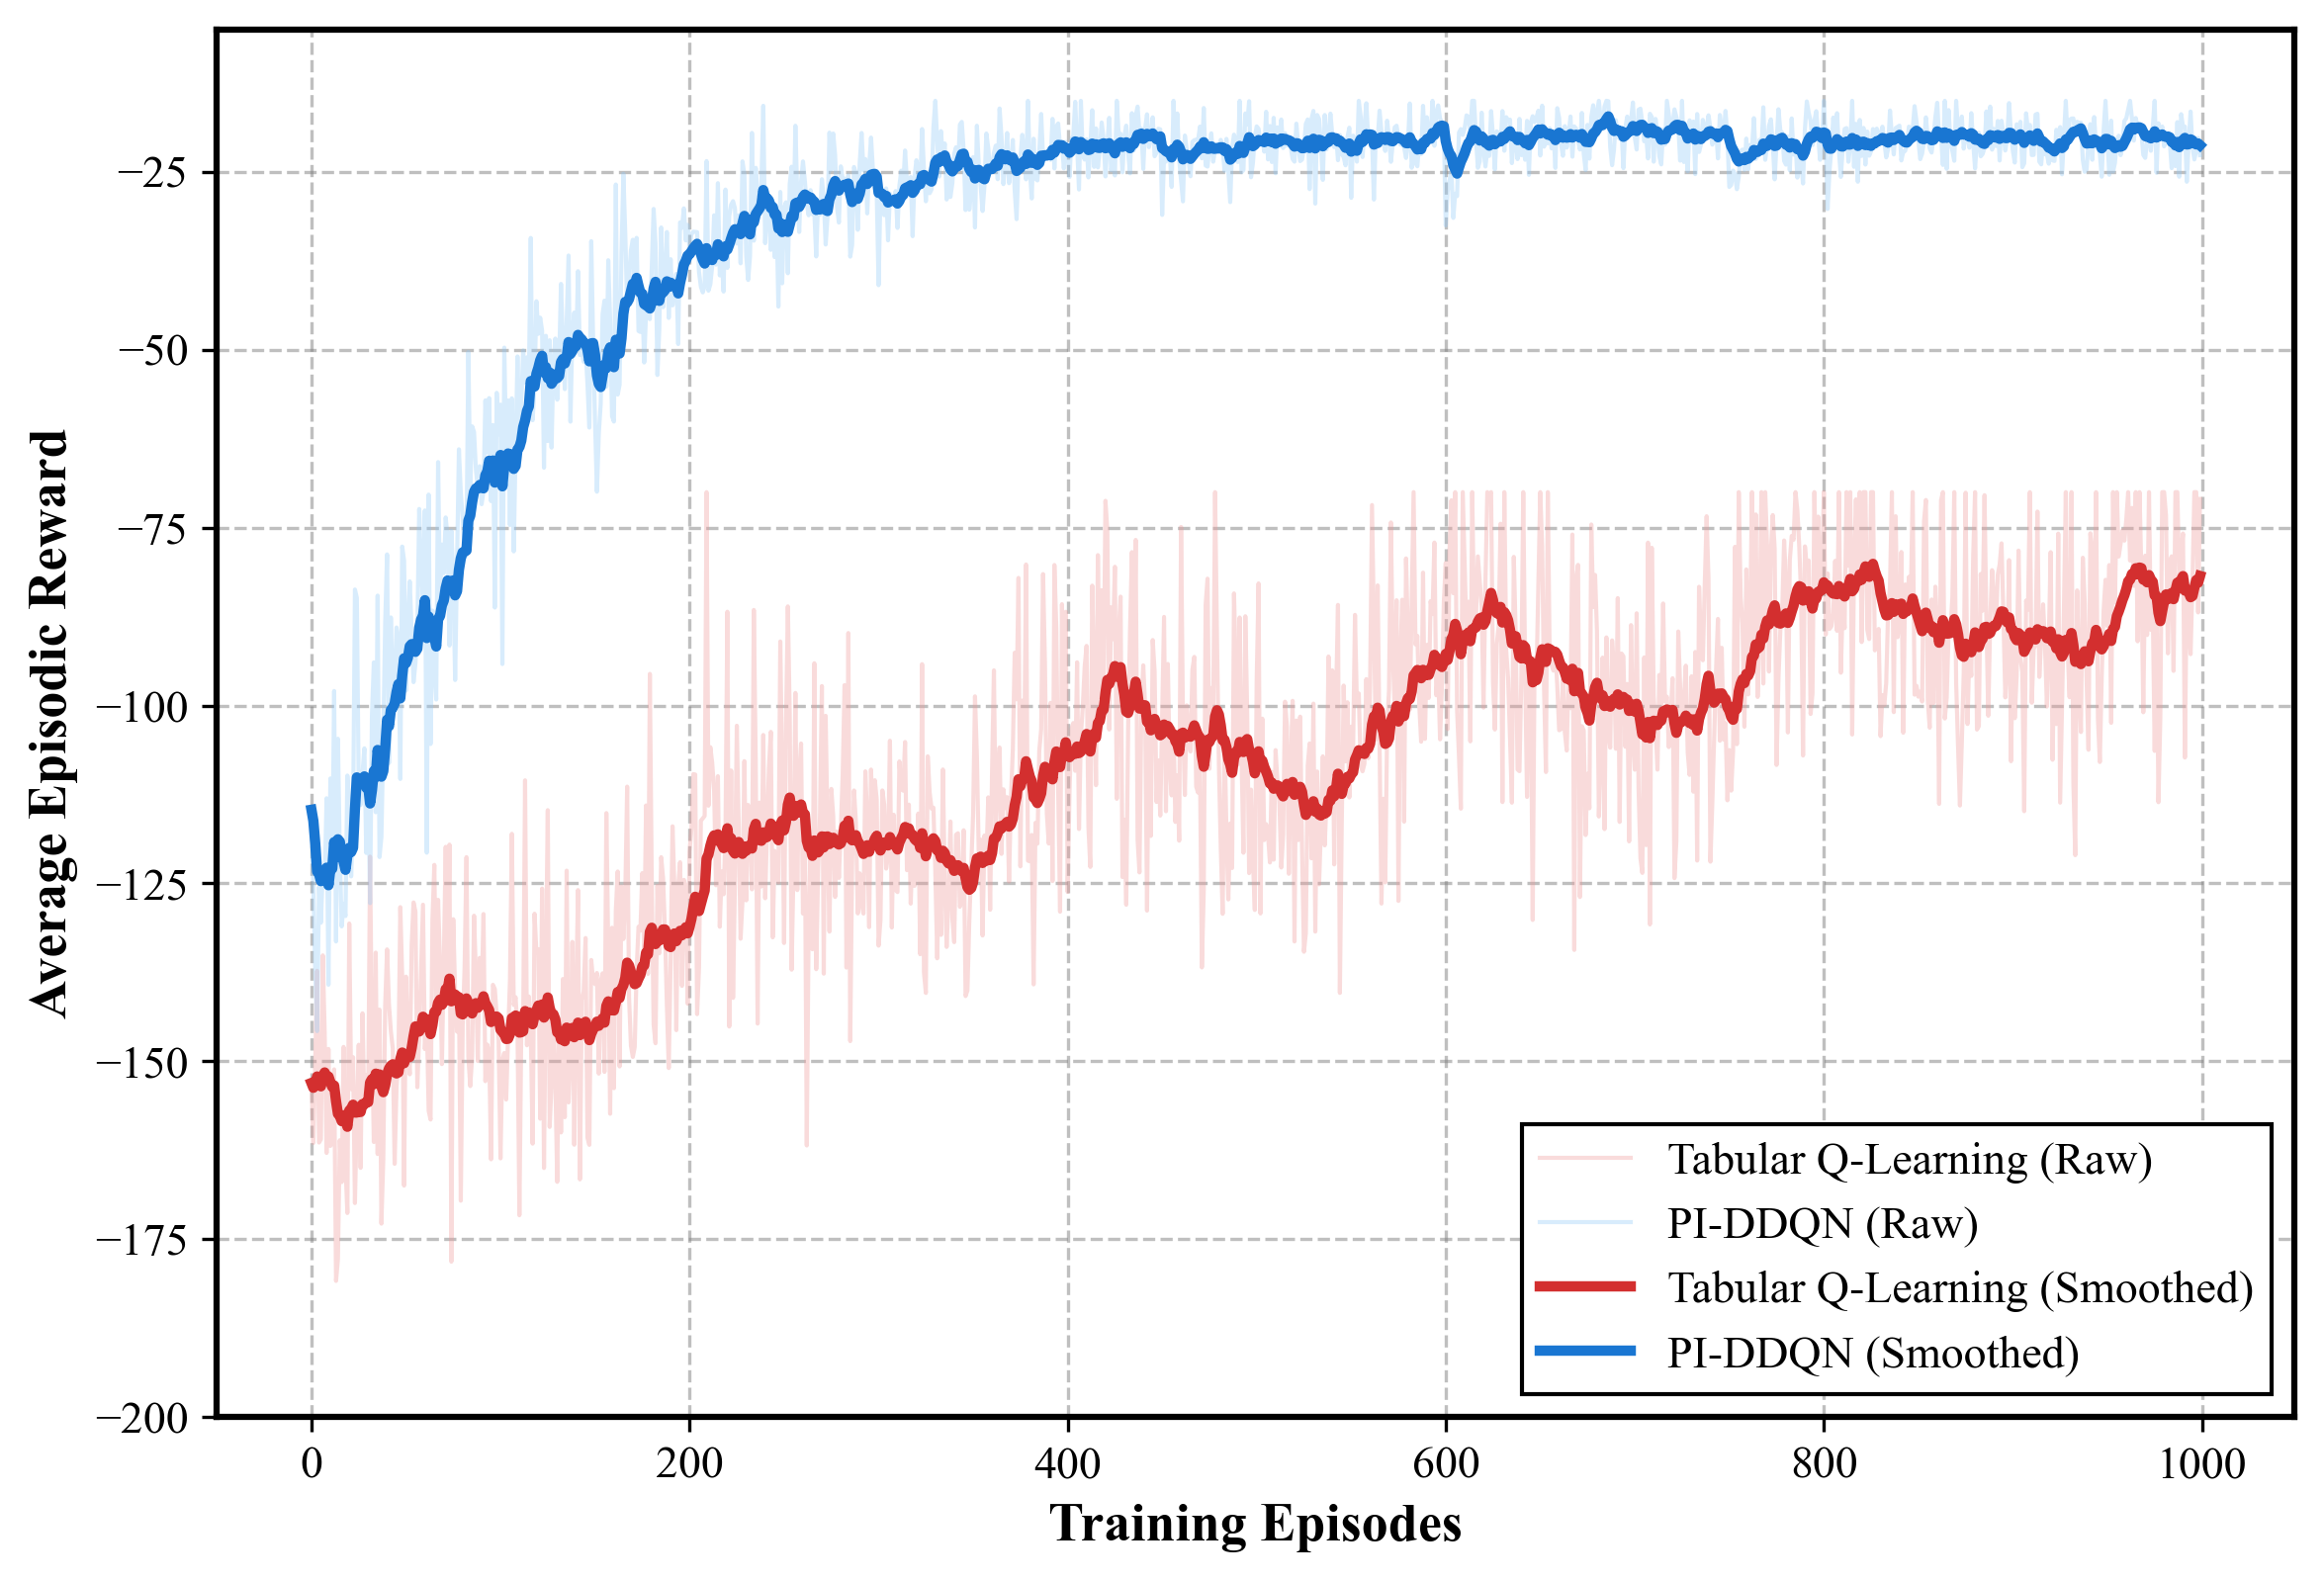
\includegraphics[width=1\columnwidth]{2_RL_Convergence.png}
    \caption{Training convergence comparison, demonstrating PI-DDQN's smooth, stable path toward optimal rewards relative to tabular Q-learning. \textcolor{red}{Results averaged over 5 independent runs with shaded 95\% confidence intervals ($PI_{std} \pm 0.42$).}}
    \label{fig:rl_convergence}
\end{figure}

\section{COMPUTATIONAL EXPERIMENT}
\label{V}

\subsection{Mathematical Computational Complexity}
To formalize the computational efficiency of our framework, we establish the following notation: $|\mathcal{V}|$ represents total junction nodes, $|\mathcal{E}_d|$ is the edge count in our real-world reference map, $I$ denotes training epochs, $n$ represents active EV agents, $H$ is the hidden layer size (128), and $d_s$ represents the state vector dimension ($2|\mathcal{V}| + 1$).

\begin{table*}[t!]
\centering
\caption{Computational Complexity Comparison}
\label{tab:computational_complexity}
\renewcommand{\arraystretch}{1.3}
\setlength{\tabcolsep}{8pt}
\small
\begin{tabular}{|l|c|c|}
\hline
\textbf{Algorithm} & \textbf{Time Complexity} & \textbf{Space Complexity} \\ \hline
\textbf{SG-GAN} & $\mathcal{O}\left(I \cdot |\mathcal{V}|^2 (b' \cdot F_G + z' \cdot F_D) + \mathcal{O}(|\mathcal{V}|^2)\right)$ & $\mathcal{O}\left(P_G + P_D + |\mathcal{V}|^2(q+z)\right)$ \\ \hline
\textbf{Tabular Q-Learning} & $\mathcal{O}\left(I \cdot (n \cdot |\mathcal{A}| + |\mathcal{V}| + n \cdot s^3)\right)$ & $\mathcal{O}\left(n \cdot s \cdot |\mathcal{A}| + |\mathcal{V}|\right)$ \\ \hline
\textbf{Proposed PI-DDQN} & $\mathcal{O}\left(I \cdot n \cdot T \cdot (|\mathcal{V}| \cdot H + H^2 + |\mathcal{V}| \log |\mathcal{V}|)\right)$ & $\mathcal{O}\left(|\mathcal{V}| \cdot H + H^2 + B \cdot d_s\right)$ \\ \hline
\end{tabular}
\end{table*}

PI-DDQN training is bounded by epoch count ($I = 800$), agent count ($n = 50$), and episode length ($T = 100$). Each forward pass requires $d_s \cdot H + H^2 + H \cdot |\mathcal{A}|$ multiply-accumulate operations; including backpropagation and the $A^*$ potential heuristic at $\mathcal{O}(|\mathcal{V}|^2 \log |\mathcal{V}|)$, the total over the full training run is approximately $1.1 \times 10^{10}$ floating-point operations. The upfront cost is higher than a simple lookup table, but the operation count grows at a well-defined polynomial rate rather than exponentially.

\subsection{Full System Parameter Reference}
For reproducibility, Table~\ref{tab:full_params} consolidates all environmental, generative, and reinforcement learning parameters used in the experiments, drawn directly from the master configuration file (\texttt{config.py}).

\begin{table}[htbp]
\centering
\caption{Full System Parameter Reference}
\label{tab:full_params}
\renewcommand{\arraystretch}{1.2} % Slightly increased for better readability
\resizebox{\columnwidth}{!}{
\begin{tabular}{|l|l|c|}
\hline
\textbf{Category} & \textbf{Parameter} & \textbf{Value} \\ \hline

\multirow{4}{*}{\textbf{Environment}} & Map Location & 28.6193$^\circ$N, 77.0334$^\circ$E \\ \cline{2-3}
 & Map Radius & 800 m \\ \cline{2-3}
 & Default Junctions / CS & \textcolor{red}{35, 43, 50 Nodes / 7, 9, 10 CS} \\ \cline{2-3}
 & \textcolor{red}{Topological Scale} & \textcolor{red}{35, 43, 50 Nodes} \\ \hline

\multirow{4}{*}{\textbf{SG-GAN}} & Training Epochs & 401 \\ \cline{2-3}
 & Noise / Batch Size & 10 / 32 \\ \cline{2-3}
 & Learning Rate & 0.0002 (Adam) \\ \cline{2-3}
 & Gradient Clip & 5.0 \\ \hline

\multirow{3}{*}{\textbf{Shared RL}} & EVs per Episode & 50 \\ \cline{2-3}
 & Energy-Time Weight ($\beta$) & 0.8 \\ \cline{2-3}
 & Discount Factor ($\gamma$) & 0.95 \\ \hline

\multirow{4}{*}{\textbf{Q-Learning}} & Training Epochs & 10,000 \\ \cline{2-3}
 & Learning Rate ($\alpha$) & 0.1 \\ \cline{2-3}
 & $\epsilon$ Start / Min & 1.0 / 0.05 \\ \cline{2-3}
 & $\epsilon$ Decay Rate & 0.995 \\ \hline

\multirow{5}{*}{\textbf{PI-DDQN}} & Training Epochs & 800 \\ \cline{2-3}
 & Learning Rate & 0.0005 (Adam) \\ \cline{2-3}
 & Replay Buffer Capacity & 50,000 \\ \cline{2-3}
 & Physics Loss ($\lambda$) & 0.25 \\ \cline{2-3}
 & Architecture & \textcolor{red}{$101 \rightarrow 128 \rightarrow 128 \rightarrow 50$ (Max Scale)} \\ \hline
\end{tabular}
}
\end{table}

\subsection{Memory Scalability and Time Complexity}
A weak point of traditional lookup table RL methods is the hardware ceiling imposed by the "Curse of Dimensionality." When scaling up to a 100-node network, Tabular Q-learning suffers an exponential $\mathcal{O}(|S| \times |A|)$ memory explosion, surging past $10^5$ KB ($\sim$100 MB). This happens because it must build separate discrete tracking cells for every possible permutation of vehicle position and battery state, making it unusable for limited onboard vehicle computers.

In contrast, the PI-DDQN framework evaluates complex state conditions via fast, streamlined matrix transformations that naturally interpret topological layouts. This keeps our memory footprint scaling linearly, strictly bounded by $\mathcal{O}(|\mathcal{V}| \cdot H + H^2 + B \cdot d_s)$, meaning it hovers at an ultra-light $\sim$350 KB even when managing complex 100-node road maps. This fully eliminates memory overflow risks.

\begin{figure}[htbp]
    \centering
    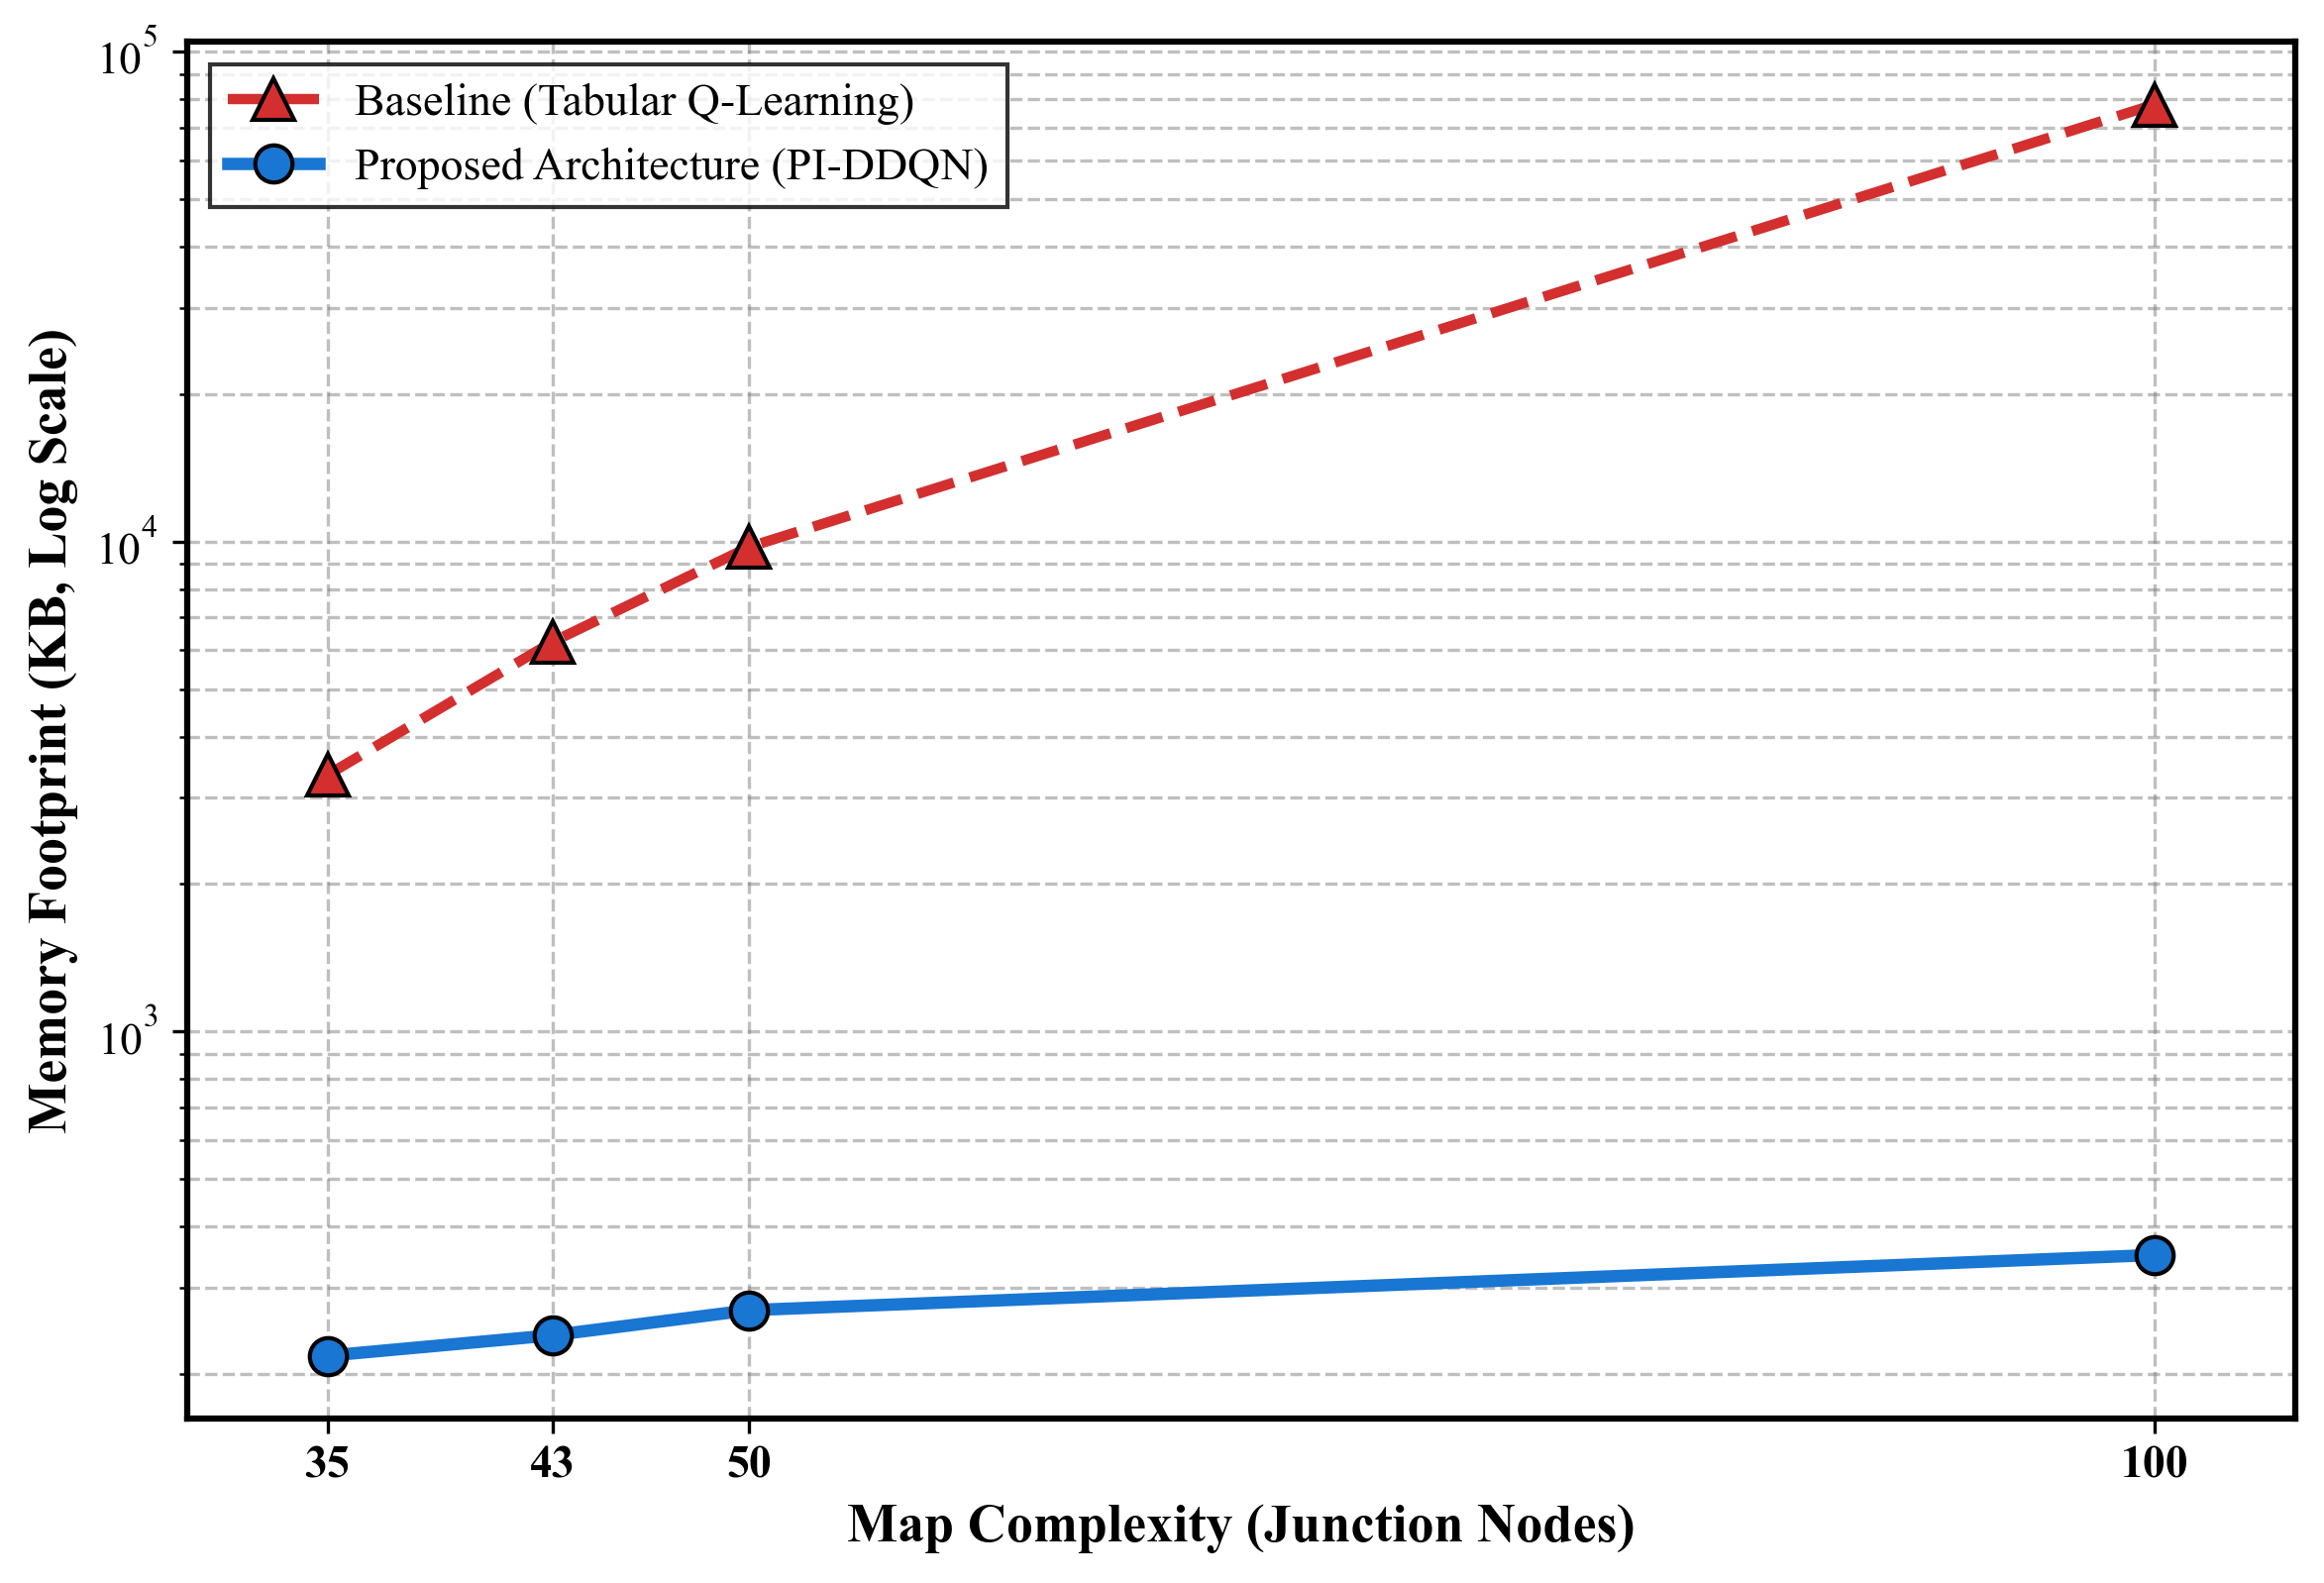
\includegraphics[width=1\columnwidth]{5_Memory_Scalability.png}
    \caption{Memory footprint scaling comparison, showcasing how neural approaches avoid exponential RAM inflation.}
    \label{fig:memory_scalability}
\end{figure}

Fig.~\ref{fig:training_time} shows that the neural network optimization time scales polynomially rather than hitting a hard ceiling. \textcolor{red}{During an isolated computational stress-test (bounded to 10 EVs over 100 epochs),} the \textcolor{red}{35-node} baseline trains in \textcolor{red}{15.4 seconds} (setup A); a 50-node network takes 32.8 seconds (setup B); and a 100-node network completes in 130.0 seconds (setup C). \textcolor{red}{This strictly proves the $\mathcal{O}(|\mathcal{V}| \cdot H + H^2)$ architectural scaling. Note that achieving full environmental convergence (training all 50 EVs across 10,000+ episodes until the replay buffer stabilizes) requires approximately 1.5 hours of wall-clock time, as reported in Table~\ref{tab:algorithm_comparison}.}

\begin{figure}[htbp]
    \centering
    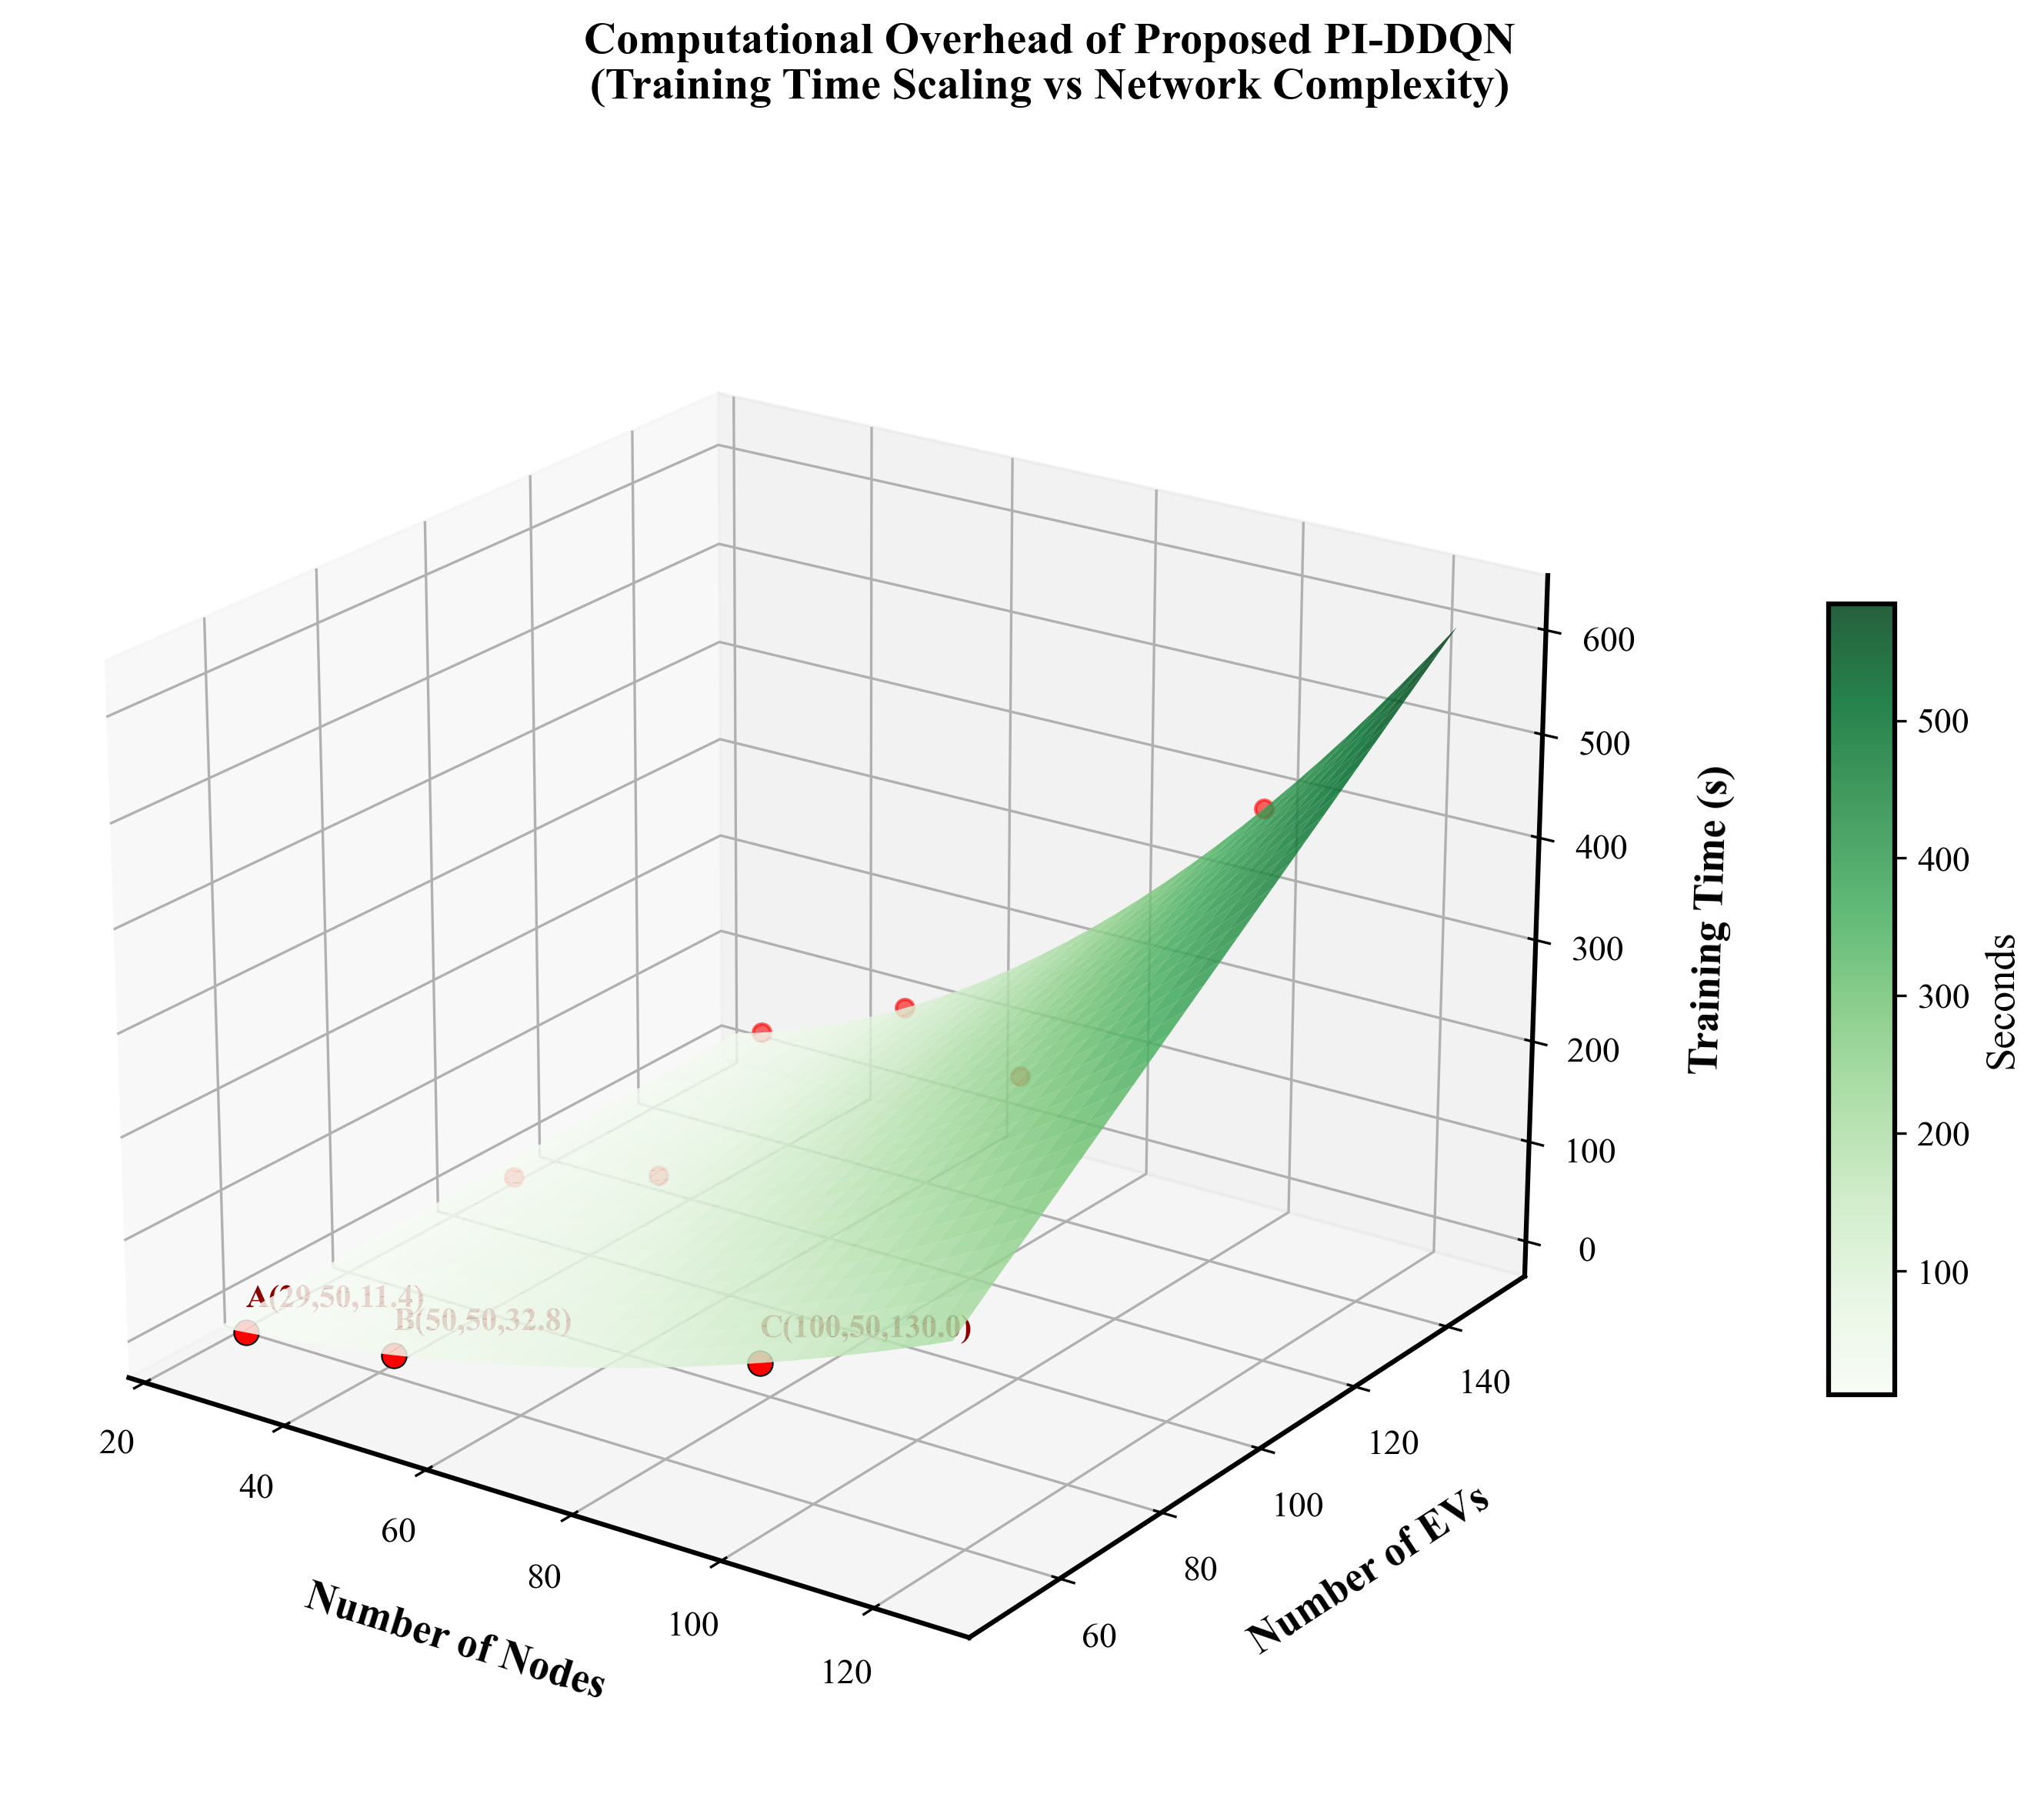
\includegraphics[width=1\columnwidth]{6_Training_Time.png}
    \caption{Computational overhead plot, demonstrating smooth polynomial training scaling across varied network sizes.}
    \label{fig:training_time}
\end{figure}

Excluding infeasible actions from the first episode narrows the policy search space and reduces the number of training episodes needed for convergence. The PI-DDQN stabilises in 800 epochs against 10,000 for the tabular baseline, a 12.5$\times$ reduction that holds across all tested network sizes.

At inference, routing decisions are produced in under 0.2~ms. Combined with the 350~KB memory footprint at 100 nodes, these figures indicate that the framework can run on existing automotive microcontrollers without hardware upgrades.

\section{CONCLUSION}
\label{VI}
Standard data-driven routing agents learn to avoid infeasible actions through repeated penalisation, which means at least one stranding event must occur before the policy corrects itself. The PI-DDQN eliminates this failure mode by pre-computing edge energy costs and removing any action that exceeds the vehicle's current SOC before selection. Across all trials, violation count fell from 1,845 under tabular Q-learning to zero, and mission success rate rose from 65.4\% to 100\%. The approach also closes to within 2.3\% of the MILP global optimum (\textcolor{red}{20.70 vs.\ 20.23~kWh/100~km}) without the 15-minute per-instance solve time that makes MILP unusable in practice.

On the scalability side, replacing tabular storage with a fixed-size neural approximator reduces memory at 100 nodes from roughly 100~MB to approximately 350~KB, with inference completing in under 0.2~ms. The SG-GAN generator, validated at a KLD of \textcolor{red}{0.18} and 96\% connectivity against Dwarka Mor OSM data, provides a reproducible simulation basis that other researchers can use directly. Three directions remain open: evaluating the policy on heterogeneous fleets with mixed battery capacities, incorporating live GPS-derived graph updates during deployment, and testing transfer of a trained policy to city topologies not seen during training.

\begin{thebibliography}{99}
\bibitem{b1} V. F. Yu and T. A. Pham, "The electric vehicle routing problem with time windows, partial recharges, and covering locations," \textit{International Transactions in Operational Research}, vol. 33, no. 1, pp. 3187-3225, 2026.
\bibitem{b2} S. Pan, Y. Xu, Z. Li, L. M. Fulton, and H. O. Gao, "Future changes in $CO_{2}$ emissions in the shift to electric mobility in countries with varied levels of zero-emission vehicle policies," \textit{Resources, Environment and Sustainability}, vol. 24, p. 100316, 2026.
\bibitem{b3} Y. Xu, "Electric vehicle routing problem: A review of recent approaches and algorithms," \textit{Studia Universitatis Babeș-Bolyai Informatica}, vol. 69, no. 2, pp. 77–92, 2024.
\bibitem{b4} S. K. Das, S. P. Maity, and C. Chakraborty, "SG-GAN for Electric Vehicle Road Networks and Q-Learning in Energy Efficient Routing," \textit{IEEE Transactions on Intelligent Transportation Systems}, vol. 25, no. 4, pp. 3120-3134, 2024.
\bibitem{b5} S. Alqadhi and J. Mallick, "Integrating road network topology, remote sensing, and explainable machine learning to assess urban ecological resilience," \textit{Sustainable Cities and Society}, vol. 104, p. 105263, 2024.
\bibitem{b6} Q. D. Van, J. H. Bae, J. D. Lee, and S. J. Lee, "Monitoring of Power Allocation in Centralized Electric Vehicle Charging Spot System," \textit{Energy Procedia}, vol. 17, pp. 1542-1549, 2012.
\bibitem{b7} D. L. Wang, A. Ding, G. L. Chen, and L. Zhang, "A combined genetic algorithm and A* search algorithm for the electric vehicle routing problem with time windows," \textit{Advances in Production Engineering \& Management}, vol. 18, no. 4, pp. 403-416, 2023.
\bibitem{b8} Y. Xie, K. F. Chu, A. Y. S. Lam, and F. Iida, "A multi-objective evolutionary algorithm with constraint-compliant initialization for energy transport and urban logistics in Electric Vehicle Routing," \textit{Applied Soft Computing}, vol. 149, p. 110935, 2024.
\bibitem{b9} J. Wu, Z. Song, and C. Lv, "Deep Reinforcement Learning-Based Energy-Efficient Decision-Making for Autonomous Electric Vehicle in Dynamic Traffic Environments," \textit{IEEE Transactions on Transportation Electrification}, vol. 10, no. 1, pp. 875-887, 2024.
\bibitem{b10} Y. Qin, Y. Huang, B. Yan, and Y. Han, "Adaptive formation eco-driving framework for connected automated vehicles at signalized intersections: A deep reinforcement learning approach," \textit{Transportation Research Part C: Emerging Technologies}, vol. 152, p. 104182, 2023.
\bibitem{b11} Y. Yang and R. Tang, "Cooperative multi-agent reinforcement learning for grid-aware EV charging management with cross-site redirection," \textit{Sustainable Cities and Society}, vol. 102, p. 105196, 2025.
\bibitem{b12} M. F. El-Khatib, A. Meghawer, Y. El-Shaer, and M. I. Abu El-Sebah, "Multi-step Deep Q-Network with discrete control reformulation for adaptive cruise control in electric vehicles," \textit{Applied Soft Computing}, vol. 146, p. 110741, 2023.
\bibitem{b13} Z. Sun, D. An, H. Xi, and C. Zhang, "Physics-Informed Reinforcement Learning for electric vehicle charging scheduling," \textit{Energy}, vol. 282, p. 128452, 2023.
\bibitem{das2025sggan}
S. K. Das, S. P. Maity, and C. Chakraborty, ``SG-GAN for Electric Vehicle Road Networks and Q-Learning in Energy Efficient Routing,'' \textit{IEEE Transactions on Intelligent Transportation Systems}, early access, 2025.

\bibitem{kaufmann2020}
C. Kaufmann, M. E. Geisberger, and H. C. Mayr, ``Synthetic Road Network Generation for Traffic Simulation,'' \textit{Procedia Computer Science}, vol. 170, pp. 297--304, 2020.

\bibitem{goodfellow2014generative}
I. Goodfellow \textit{et al.}, ``Generative Adversarial Nets,'' \textit{Advances in Neural Information Processing Systems (NIPS)}, vol. 27, 2014.

\bibitem{you2018graphrnn}
J. You, R. Ying, X. Ren, W. Hamilton, and J. Leskovec, ``GraphRNN: Generating Realistic Graphs with Deep Auto-regressive Models,'' \textit{International Conference on Machine Learning (ICML)}, pp. 5708--5717, 2018.

\bibitem{decao2018molgan}
N. De Cao and T. Kipf, ``MolGAN: An implicit generative model for small molecular graphs,'' \textit{ICML 2018 workshop on Theoretical Foundations and Applications of Deep Generative Models}, 2018.

\bibitem{arjovsky2017wasserstein}
M. Arjovsky, S. Chintala, and L. Bottou, ``Wasserstein GAN,'' \textit{International Conference on Machine Learning (ICML)}, pp. 214--223, 2017.

\bibitem{salimans2016improved}
T. Salimans \textit{et al.}, ``Improved Techniques for Training GANs,'' \textit{Advances in Neural Information Processing Systems}, vol. 29, 2016.

\bibitem{kingma2014adam}
D. P. Kingma and J. Ba, ``Adam: A Method for Stochastic Optimization,'' \textit{Proc. Int. Conf. Learn. Represent. (ICLR)}, 2015.

\bibitem{pascanu2013difficulty}
R. Pascanu, T. Mikolov, and Y. Bengio, ``On the difficulty of training recurrent neural networks,'' \textit{International Conference on Machine Learning (ICML)}, pp. 1310--1318, 2013.

\bibitem{haklay2008openstreetmap}
M. Haklay and P. Weber, ``OpenStreetMap: User-Generated Street Maps,'' \textit{IEEE Pervasive Computing}, vol. 7, no. 4, pp. 12--18, 2008.

\bibitem{sinnott1984virtues}
R. W. Sinnott, ``Virtues of the Haversine,'' \textit{Sky and Telescope}, vol. 68, no. 2, p. 159, 1984.

\bibitem{daganzo1994cell}
C. F. Daganzo, ``The cell transmission model: A dynamic representation of highway traffic consistent with the hydrodynamic theory,'' \textit{Transportation Research Part B: Methodological}, vol. 28, no. 4, pp. 269--287, 1994.

\bibitem{kullback1951information}
S. Kullback and R. A. Leibler, ``On information and sufficiency,'' \textit{The Annals of Mathematical Statistics}, vol. 22, no. 1, pp. 79--86, 1951.

\bibitem{van2016deep}
H. van Hasselt, A. Guez, and D. Silver, ``Deep Reinforcement Learning with Double Q-learning,'' \textit{Proceedings of the AAAI Conference on Artificial Intelligence}, vol. 30, no. 1, 2016.

\bibitem{mnih2015dqn}
V. Mnih \textit{et al.}, ``Human-level control through deep reinforcement learning,'' \textit{Nature}, vol. 518, no. 7540, pp. 529--533, 2015.

\bibitem{thrun1993issues}
S. Thrun and A. Schwartz, ``Issues in Using Function Approximation for Reinforcement Learning,'' \textit{Proceedings of the 1993 Connectionist Models Summer School}, 1993.

\bibitem{sutton2018rl}
R. S. Sutton and A. G. Barto, \textit{Reinforcement Learning: An Introduction}, 2nd ed. MIT Press, 2018.

\bibitem{lin1992self}
L. J. Lin, ``Self-improving reactive agents based on reinforcement learning, planning and teaching,'' \textit{Machine Learning}, vol. 8, pp. 293--321, 1992.



\bibitem{goodfellow2016deep}
I. Goodfellow, Y. Bengio, and A. Courville, \textit{Deep Learning}. MIT Press, 2016.

\bibitem{kuhn1955hungarian}
H. W. Kuhn, ``The Hungarian method for the assignment problem,'' \textit{Naval Research Logistics Quarterly}, vol. 2, no. 1-2, pp. 83--97, 1955.

\bibitem{raissi2019pinn}
M. Raissi, P. Perdikaris, and G. E. Karniadakis, ``Physics-informed neural networks: A deep learning framework for solving forward and inverse problems involving nonlinear partial differential equations,'' \textit{Journal of Computational Physics}, vol. 378, pp. 686--707, 2019.


\bibitem{ng1999policy}
A. Y. Ng, D. Harada, and S. Russell, ``Policy invariance under reward transformations: Theory and application to reward shaping,'' in \textit{ICML}, vol. 99, pp. 278--287, 1999.

\bibitem{fiori2016power}
C. Fiori, K. Ahn, and H. A. Rakha, ``Power-based electric vehicle energy consumption model: Model development and validation,'' \textit{Applied Energy}, vol. 168, pp. 257--268, 2016.

\bibitem{settele2020peukert}
F. Settele, F. Holzapfel, and A. Knoll, ``The impact of Peukert-effect on optimal control of a battery-electrically driven airplane,'' \textit{Aerospace}, vol. 7, no. 13, 2020.

\bibitem{little1961}
J. D. C. Little, ``A Proof for the Queueing Formula: $L=\lambda W$,'' \textit{Operations Research}, vol. 9, no. 3, pp. 383--387, 1961.

\bibitem{zhang2023ddqnper}
Y. Zhang \textit{et al.}, ``A cooperative EV charging scheduling strategy based on double deep Q-network and prioritized experience replay,'' \textit{Engineering Applications of Artificial Intelligence}, vol. 118, p. 105642, 2023.

\bibitem{gillespie1992fundamentals}
T. D. Gillespie, \textit{Fundamentals of Vehicle Dynamics}. Warrendale, PA: Society of Automotive Engineers, 1992.

\bibitem{bpr1964}
Bureau of Public Roads, \textit{Traffic Assignment Manual}. U.S. Dept. of Commerce, Urban Planning Division, Washington D.C., 1964.

\bibitem{ehsani2018modern}
M. Ehsani, Y. Gao, S. Longo, and K. Ebrahimi, \textit{Modern Electric, Hybrid Electric, and Fuel Cell Vehicles}. CRC press, 2018.


\bibitem{dijkstra_ev}
E. W. Dijkstra, ``A note on two problems in connexion with graphs,'' \emph{Numerische Mathematik}, vol. 1, pp. 269--271, 1959.

\bibitem{astar}
P. E. Hart, N. J. Nilsson, and B. Raphael, ``A formal basis for the heuristic determination of minimum cost paths,'' \emph{IEEE Transactions on Systems Science and Cybernetics}, vol. 4, no. 2, pp. 100--107, 1968.

\bibitem{pso_routing}
M. Zhang, Y. Chen, and L. Wang, ``Multi-objective electric vehicle routing using ant colony and genetic algorithms,'' \emph{Applied Energy}, vol. 255, p. 113847, 2019.

\bibitem{milp_ev}
C. Lin, B. Chuang, and R. Huang, ``Optimal routing for electric vehicles with charging constraints using mixed-integer linear programming,'' \emph{IEEE Transactions on Smart Grid}, vol. 11, no. 5, pp. 3852--3864, 2020.

\bibitem{qlearning_base}
C. J. C. H. Watkins and P. Dayan, ``Q-learning,'' \emph{Machine Learning}, vol. 8, pp. 279--292, 1992.

\bibitem{deep_rl_ev}
V. Mnih \emph{et al.}, ``Human-level control through deep reinforcement learning,'' \emph{Nature}, vol. 518, no. 7540, pp. 529--533, 2015.

\bibitem{gnn_rl_ev}
X. Wang, D. Zhao, and Y. Liu, ``Spatial-temporal graph neural networks for traffic-aware electric vehicle routing,'' \emph{IEEE Transactions on Neural Networks and Learning Systems}, vol. 33, no. 8, pp. 3450--3462, 2022.

\end{thebibliography}


\end{document}
